\documentclass[a4paper, 11pt, twoside]{tesis}

\usepackage[utf8]{inputenc}
\usepackage[spanish]{babel}
\usepackage{graphicx}
\usepackage[space]{grffile}
\usepackage{caption}
\usepackage{subcaption}
\usepackage{xspace}
\usepackage{cite}
\usepackage{listings}
\usepackage[colorinlistoftodos, shadow]{todonotes}
\usepackage{amsmath}
\usepackage{amsthm}
\usepackage{paralist}
\usepackage{wrapfig}
\usepackage{booktabs}
\usepackage{url}
\usepackage{titlesec}
\usepackage{color, colortbl}
\usepackage{amsmath}
\usepackage{rotating}
% \usepackage{hyperref}

\titleformat*{\subsubsection}{\bfseries}
% \usepackage[disable]{todonotes}

\begin{document}

%%% Definiciones de formato
\newcommand{\mc}{\emph{Model Checking}\xspace}
\newcommand{\smc}{\emph{Symbolic Model Checking}\xspace}
\newcommand{\bmc}{\emph{Bounded Model Checking}\xspace}

\newcommand{\bdd}{\emph{Binary Decision Diagram}\xspace}
\newcommand{\bdds}{\emph{Binary Decision Diagrams}\xspace}

\newcommand{\ssolver}{\emph{sat-solver}\xspace}
\newcommand{\ssolvers}{\emph{sat-solvers}\xspace}
\newcommand{\ssolving}{\emph{sat-solving}\xspace}

\newcommand{\bcp}{\emph{Boolean Constraint Propagation}\xspace}
\newcommand{\BCP}{\texttt{BCP}\xspace}

\newcommand{\T}{\textbf{\texttt{True}}\xspace}
\newcommand{\F}{\textbf{\texttt{False}}\xspace}

\newcommand{\true}{\texttt{TRUE}\xspace}
\newcommand{\false}{\texttt{FALSE}\xspace}
\newcommand{\sat}{\emph{sat}\xspace}
\newcommand{\unsat}{\emph{unsat}\xspace}
\newcommand{\cnf}{\texttt{\textbf{CNF}}\xspace}
\newcommand{\npc}{\textbf{NP-Complete}\xspace}
\newcommand{\bt}{\emph{backtracking}\xspace}
\newcommand{\gp}{\emph{guiding path}\xspace}

\newcommand{\dpll}{\texttt{DPLL}\xspace}
\newcommand{\cdcl}{\emph{Conflict Driven Clause Learning}\xspace}
\newcommand{\CDCL}{\texttt{CDCL}\xspace}

\newcommand{\soft}{\emph{software}\xspace}
\newcommand{\hard}{\emph{hardware}\xspace}

\newcommand{\cluster}{\emph{cluster}\xspace}

\newcommand{\w}{\emph{worker}\xspace}
\newcommand{\ws}{\emph{workers}\xspace}

\newcommand{\solveando}{\emph{solveando}\xspace}
\newcommand{\solvear}{\emph{solvear}\xspace}
\newcommand{\solveado}{\emph{solveado}\xspace}
\newcommand{\solving}{\emph{solving}\xspace}
\newcommand{\ots}{\emph{off-the-shelf}\xspace}
\newcommand{\Python}{\texttt{Python}\xspace}
\newcommand{\minisatdosveinte}{\texttt{Minisat 2.2.0}\xspace}
\newcommand{\minisat}{\texttt{Minisat}\xspace}
\newcommand{\cpp}{\texttt{C++}\xspace}
\newcommand{\mpi}{\texttt{MPI}\xspace}

\newcommand{\bend}{\emph{backend}\xspace}
\newcommand{\fend}{\emph{frontend}\xspace}

\newcommand{\datapath}{\emph{datapath}\xspace}
\newcommand{\thread}{\emph{thread}\xspace}
\newcommand{\threads}{\emph{threads}\xspace}

\newcommand{\io}{\texttt{I/O}\xspace}
\newcommand{\cpu}{\texttt{CPU}\xspace}

\newcommand{\clusters}{\emph{clusters}\xspace}

\newcommand{\tout}{\emph{timeout}\xspace}

\newcommand{\masterslave}{\texttt{Master-Worker}\xspace}
\newcommand{\master}{\emph{MasterProxy}\xspace}

\newcommand{\lst}{List.~}
\newcommand{\fig}{Fig.~}

\newcommand{\rt}{\emph{run-time}\xspace}
\newcommand{\apriori}{\emph{a priori}\xspace}

%%%% CARATULA
\def\autor{Ignacio Vissani}
\def\titulo{Un \ssolver paralelo y distribuido con herencia de cláusulas aprendidas} 
\def\runtitulo{Un \ssolver paralelo y distribuido con herencia de cláusulas aprendidas}
\def\runtitle{A parallel and distributed \ssolver with learned clauses inheritance}
\def\director{Nicolás Leandro Rosner}
\def\codirector{Carlos Gustavo López Pombo}
\def\lugar{Buenos Aires, 2013}

\newcommand{\HRule}{\rule{\linewidth}{0.2mm}}
%
\thispagestyle{empty}

\begin{center}\leavevmode

\vspace{-2cm}

\begin{tabular}{l}

\includegraphics[width=2.6cm]{logofcen.pdf}
\end{tabular}


{\large \sc Universidad de Buenos Aires

Facultad de Ciencias Exactas y Naturales

Departamento de Computaci\'on}

\vspace{6.0cm}

%\vspace{3.0cm}
%{
%\Large \color{red}
%\begin{tabular}{|p{2cm}cp{2cm}|}
%\hline
%& Pre-Final Version: \today &\\
%\hline
%\end{tabular}
%}
%\vspace{2.5cm}

{\huge\bf \titulo}

\vspace{2cm}

{\large Tesis presentada para optar al t\'{\i}tulo de\\
Licenciado en Ciencias de la Computaci\'on}

\vspace{2cm}

{\Large \autor}

\end{center}

\vfill

{\large

{Director: \director}

\vspace{.2cm}

{Codirector: \codirector}

\vspace{.2cm}

\lugar
}

\newpage\thispagestyle{empty}


%%%% ABSTRACTS, AGRADECIMIENTOS Y DEDICATORIA
\frontmatter
\pagestyle{empty}
%!TEX root = tesis.tex

%\begin{center}
%\large \bf \runtitulo
%\end{center}
%\vspace{1cm}
\chapter*{\runtitulo}

En la actualidad el \soft forma parte integral de nuestra vida. Este interviene 
en todo tipo de tareas. Desde el envío de un mensaje de texto
o la realización de una llamada telefónica hasta el sistema de control de una
central nuclear o el sistema de velocidad crucero de un automóvil, utilizan sistemas basados en \hard y \soft
informático. 

El análisis de software es un área en la ingeniería de software que en general se ocupa de la aplicación de métodos formales que permiten garantizar, o al menos ganar confianza en, la ausencia de errores en una pieza de \soft. Existe una plétora de herramientas dedicadas a esta tarea, cada una de ellas con sus elecciones particulares de lenguajes y método a aplicar. Entre ellas, una cantidad no menor se ha volcado al uso de \ssolvers \emph{off-the-shelf} como mecanismo de bajo nivel que permite explorar eficientemente un espacio finito de modelos. 

En el presente trabajo pretende implementar un \ssolver paralelo y distribuido que:
\begin{inparaenum}[a)]  
\item realice una adecuación y balanceo de la carga de procesamiento en \emph{run-time} sobre una cantidad y configuración de equipamiento desconocida,
\item realice una adecuación y balanceo del uso de memoria primaria y secundaria en \emph{run-time}, también sobre una cantidad y configuración de equipamiento desconocida, y 
\item sea extensible y fácil de parametrizar en todos aquellos aspectos que determinen el comportamiento del procedimiento de resolución del problema. 
\end{inparaenum}
Una vez llevada a cabo esta tarea, se pretende evaluar la viabilidad de implementar una técnica de aprendizaje basada en análisis de cláusulas de conflicto acorde a las necesidades de ambientes paralelos y distribuidos, y su comparación empírica.

\bigskip

\noindent\textbf{Palabras claves:} Software engineering, Verificación and validación, Sat-solvers, Parallelo y distribuido, Aprendizaje basado en conflictos.

%\cleardoublepage
%!TEX root = tesis.tex

%\begin{center}
%\large \bf \runtitle
%\end{center}
%\vspace{1cm}
\chapter*{\runtitle}

Software is nowadays an integral part of our lives. It participates in all
kind of tasks. From the sending of a text message or the realisation of a
phone call, to the control system of a nuclear plant or the cruise control
system of a car use systems based on hardware and software.

Software analysis is a field in software engineering that in general has the
responsibility of the application of formal methods in order to guaranty, or
at least gain some confidence in the absence of errors in a software artifact.
There exists a plethora of tools dedicated to that task, each one of them with
their particular biases for specific languages and methods to be applied.
Among them, there are many that have turn to the use of \ssolvers \emph{off-
the-shelf}  as a low level mechanism allowing the efficient exploration of a
finite space of models.
 
The aim of the present work is to implement a parallel and distributed
\ssolver that: \begin{inparaenum}[a)]   \item provides an adequate processing
workload balance at run-time over an \emph{a priori} unknown quantity and
configuration of equipment, \item provides an adequate balance of memory use,
both primary and secondary, at run-time over an unknown quantity and
configuration of equipment, \item is extensible and easy to parameterize in
all the relevant aspects that determines the behaviour of the tool in the
solution of the problem. \end{inparaenum} Once this task is done, we will
evaluate the viability of the implementation of learning techniques based in
conflict clause analysis according to the needs of parallel and distributed
scenarios, and their empirical comparison.

\bigskip

\noindent \textbf{Keywords:} Software engineering, Verification and
validation, Sat-solvers, Parallel and distributed, Conflict based learning.


%\cleardoublepage
%!TEX root = tesis.tex

\chapter*{Agradecimientos}

Intento determinar cuál fue el punto en el tiempo en el que todo empezó. No lo tengo muy claro. Mis recuerdos más viejos son para Nacho Regueira y Alejandro Abramoff. Cada uno con sus respectivas \texttt{XT} en las que hacíamos carteles con el Banner o jugábamos al Arkanoid ¿O tal vez fue en lo de Martín González? Un cumpleaños, sí. Una Commodore con un juego ¿Galaga tal vez? Después de eso, laguna, nada. Se me viene la 286, la primera compu ``mía''. Una flamante 286 con monitor color. Creo que fue un regalo de cumpleaños. Un regalo de mis viejos que era más bien para toda la familia. No recuerdo el día que llegó, pero sí recuerdo el día en que ``accidentalmente'' la \emph{formatié}. El técnico que vino aquella vez fue el primero que me enseñó algo de \emph{computación}. En aquella aprendimos Quattro Pro y Lotus123 con mi mamá. Después se me viene el lugar de los jueguitos, en el que parábamos con mi papá a veces cuando íbamos o veníamos de lo de la abuela Pocha. Creo que con el de Los Simpson nos agarramos el primer virus. El famoso Michellangelo. Me acuerdo también de cuando intenté, infructuosamente, instalarle Windows 95 a la pobre 286. Un Windows que me copié, diskette por diskette (creo que eran 16) de lo de Nadav Rajzman. Claramente nunca funcionó. En ese entonces ni me imaginaba que era imposible que funcione.

Lo próximo que recuerdo son los primeros años de la secundaria. Ya estaba cansado de la 286, que para ese entonces era más que vieja, así que me iba caminando al colegio para ahorrar hasta el último centavo de la mensualidad que me daba mi vieja. Así logré comprarme la Pentium 233 (¡con MMX!). Y con esa pasé los años en el Acosta, donde conocí a mucha gente que poco tuvo que ver con mi afinidad por la computación, pero mucho tuvo que ver con convertirme en la persona que soy, con todo lo que eso implica. La banda de Bande (en especial Mavi, Chuli, Diego, Juan, Santiago, Fede. Y Hernán, amigo de toda la vida), con la que, entre cafés con leche con dos de azucar y cervezas de \$1,60 perdimos el tiempo de la forma más maravillosa posible, entre amigos. Pepe y Manolo que siempre nos saludaban a la voz de ``Doctor''. Y pensar que algún día eso iba a tener un significado...

Después ``-¿Qué vas a estudiar?''. La pregunta más temida. ``-Ingeniería en informática...'', ``-Ajá'' y eso fue todo lo que dijo mi viejo. Tiempo después me dijo ``¿Por qué no te fijás? Hay una carrera de computación, en la facultad de Exactas, creo que se llama Computador científico...'' supongo que un arquitecto no podía permitir que su hijo fuera ingeniero. Para reforzar, en el CBC lo conocí a Damián, que estaba anotado para esa carrera de exactas en la que ``cuando entrás, lo primero que te dicen es que lo del CBC no sirve para nada, y estudiás todo de nuevo, pero bien'' ¡A mi juego me llamaron! Así llegué un día de Marzo de 2003, por primera vez, a Ciudad Universitaria. Todavía con la simultaneidad a cuestas. Y no me fui más.

Muchas cosas y mucha gente. Imposible hacerle honor a todas y todos. Aparece Damián nuevamente, consiguiéndome mi primer trabajo en el área. Él y Gutes (``el de ORT, que viene en auto''). Mi primer grupo de TP. El BebeJugando. Qué de chorizos a la pomarola, ñoquis caseros y asaditos que nos mandamos esos fines de semana de estudio entre Flores y Floresta (sin chiste por favor). Y cuando no nos juntábamos, mate en la mesa con mis hermanas, Tute, Chancho y Chuletas. Después aparecen Mati, Román, Piter, Tommy, Guido. Estábamos cursando (si se puede decir) AlgoII y empezamos a juntarnos a discutir ``cosas'' de la facultad junto con Charly y Nico Maur con quienes después fundamos la AEI. La agrupación con la que conquistamos el CoDep de computación por vaaaaarios años consecutivos. Mati y Piter de nuevo, AlgoIII. Gran cursada. Hace su aparición el piquetero programador, el remise con el TP, el té con tortas, Marmol y las pastas ¿Se acuerdan cuando nos ofendimos porque nos aprobaron un TP que claramente NO estaba bien?

Después la carrera se me va a un segundo plano. Sobresale la militancia. Itai y Fede. Charly y Nico de nuevo. Leo. Con quienes construimos una locura. A contramano y sin permiso. Con la bandera del pelado, un ``¿Por qué nacimos?¿Por qué luchamos?'' diseñado entre gallos y medianoches, a conquistar los sueños de una juventud inconforme, crítica, rebelde. Qué distante y a la vez, qué fundamental.

Y en el medio de la vorágine militante, se me aparece Ali ``esa, la que habló en la asamblea, la troska''. Resultó que troska no era. Pero sí fue (y es) mi compañera. Cuántas tardes estudiando en lo de Graciela. Bah, ella estudiaba y mientras me decía a mí ``dale, estudiá''. Cuántas noches en vela por el centro de estudiantes. Cuántos cronogramas, ajustes de cronogramas y ajustes de los ajustes de cronogramas que me armaste. Cuánta compañía, cuánta banca, cuánta paciencia, cuánto empuje. Y cuántas otras cosas para las que sobran las palabras.

Me estoy olvidando de muchos. Mis compañeros docentes. Estoy convencido de que aprendí más siendo docente que siendo estudiante. Se me vienen los que me ayudaron en mis primeros pasos: Schapa, Charly (ya dejá de aparecer che!), DFS. Aquellos con los que nos cargamos materias al hombro, Mati, Piter, Nico Rosner. La banda que hizo patria en Sistemas, Pablete, Mariano.

Los pibes del FEM!, en especial Marce con quien siempre compartimos interminables discusiones sobre la ciencia, la política científica y la historia universitaria. Manu y Nico, Lau, Lipa y Nano, Mauro, la primera camada. La CoNEAU ¿se acuerdan de la CoNEAU?

Los fieles de la bondiola. Dani V., Fran, Facu, Mica, Fede, Marianito y tantos otros de los que me estoy olvidando. Interminables comidas bajo la incumplible consigna de ``hoy no hablamos del DC''.

Toda la gente que ocupa, física o espiritualmente, la oficina 8. Mariano, Marcelo, Manu, Cani, Pau, Nico, Charly ¡Limpien el mate cuando se van!

Ya vengo llegando al final. Mis últimos recuerdos son para mis directores, Nico y Charly. Qué veranito ¡eh!

Al final, no sé en cuál de todos estos recuerdos está el punto de inflexión que me llevó hasta acá. Creo que fue un poco de todo. Lo que es seguro es que si uno de ustedes hubiera faltado, yo no habría sido el mismo, mi trabajo no habría sido el mismo. Por eso, a todos ustedes, muchas gracias. Más que muchas, infinitas. % OPCIONAL: comentar si no se quiere

\cleardoublepage
%!TEX root = tesis.tex
\hfill \textit{A mi viejo.}  % OPCIONAL: comentar si no se quiere

%\cleardoublepage
\tableofcontents

\mainmatter
\pagestyle{headings}

\theoremstyle{definition}
\newtheorem{definition}{Definición}[section]

\theoremstyle{theorem}
\newtheorem{theorem}{Teorema}[section]

\newcommand{\disj}[1]{\ensuremath{[#1]}}
\newcommand{\conj}[1]{\ensuremath{\{#1\}}}

\theoremstyle{theorem}
\newtheorem{remark}{Observación}[section]

\theoremstyle{theorem}
\newtheorem{proposition}{Proposición}[section]

\newcommand{\defname}[1]{\textbf{\emph{[#1]}}}
\newcommand{\theoname}[1]{\textbf{\emph{[#1]}}}

\listoftodos

%!TEX root = tesis.tex

\chapter{Introducción} 
\label{intro}

En la actualidad el \soft forma parte integral de nuestra vida. Este interviene en todo tipo de tareas. Desde el envío de un mensaje de texto
o la realización de una llamada telefónica hasta el sistema de control de una
central nuclear, pasando por el control de un ascensor o el sistema de
velocidad crucero de un automóvil, utilizan sistemas basados en \hard y \soft
informático. La variedad, alcance y \textbf{criticidad} de las
responsabilidades asignadas a las piezas de \soft hacen de las mismas un
componente de alto impacto en nuestra realidad cotidiana.

Por otra parte, la alta complejidad del \soft hace que la construcción del
mismo sea una tarea propensa a errores. El impacto de una falla en un
componente de \soft puede variar desde la imposibilidad de utilizar un
artefacto doméstico hasta una catástrofe de magnitudes como la fundición del
núcleo de un reactor nuclear.

Son estos aspectos los que motivan la necesidad creciente de construir métodos
(formalismos, metodologías, herramientas, etc.) que permitan garantizar la
calidad del \soft en un sentido general. La posibilidad de establecer la
ausencia de errores en un programa radica en la capacidad de establecer
inequívocamente que ese programa cumple una determinada propiedad que expresa
el adecuamiento del mismo al comportamiento esperado. Por ejemplo si
quisiéramos establecer el correcto  funcionamiento del mecanismo de seguridad
de un horno de microondas podríamos enunciar una propiedad como la siguiente:
``No es posible encender el microondas si la puerta está abierta''.

La \textbf{verificación formal} de \soft consiste en demostrar que un
determinado sistema o algoritmo es correcto respecto a una
\textbf{especificación formal} del mismo. Los lenguajes naturales son
intrínsecamente ambiguos y por lo tanto una descripción de un sistema
realizada en lenguaje natural resulta muy difícil de verificar. En lo
subsiguiente asumiremos que una especificación será formal en tanto está
descripta en un lenguaje que posee:  \begin{inparaenum}[a)]  \item reglas para
determinar cuándo una sentencia pertenece al lenguaje (sintaxis),  \item
reglas que permitan interpretar las sentencias (bien formadas) de manera
precisa y significativa (semántica), y  \item reglas para inferir información
útil a partir de la especificación (\emph{proof theory}).  \end{inparaenum}

El enfoque de la verificación formal de software, tal vez uno de los más
ambiciosos en el campo de la ingeniería de software, enfrenta dos problemas
fundamentales. En primer lugar está la dificultad de construir una
especificación formal que exprese de manera correcta el comportamiento
esperado del sistema (a lo que llamaremos validación) ya que el mismo
normalmente proviene de requerimientos expresados en lenguaje natural. El
segundo problema fundamental es que las lógicas subyacentes a la mayoría de
los lenguajes formales capaces de expresar un conjunto lo suficientemente
amplio e interesante de propiedades son normalmente indecidibles, es decir que
no existe un algoritmo capaz de, para toda fórmula del lenguaje, establecer si
la misma es un teorema o no.

El problema de la indecidibilidad se transforma en un escollo fundamental en
tanto impide la construcción de métodos de verificación formal completamente
automáticos. Diversos enfoques han sido desarrollados para atacar este
problema \todo[inline]{Buscar citas. SMT Solving, Bounded MC, etc}. La mayoría
de estos métodos consisten en restringir de alguna manera el lenguaje formal
utilizado de modo de generar un sublenguaje del mismo que sea decidible. Uno
de los enfoques desarrollados en este sentido es el conocido como \bmc
(verficación acotada de modelos).

\mc\cite{emerson:scp-2_3} es una técnica desarrollada para la verificación de
sistemas reactivos. La técnica consiste en la exploración exhaustiva y
automática del espacio de estados de un sistema modelado como una máquina de
estados finita. Cuando la cantidad de estados del sistema es relativamente
grande la exploración exhaustiva del espacio de estados se vuelve
inpracticable. Esto motivó el desarrollo de la técnica conocida como
\smc\cite{burch:lics90, mcmillan93} que ataca el problema antedicho a partir
de evitar construir el grafo de estados del sistema utilizando fórmulas
lógicas para caracterizar conjuntos y relaciones. Cuando se trata de fórmulas
proposicionales, en \smc el chequeo de las fórmulas es realizada típicamente
mediante el uso de BDDs (\bdds)\cite{bryant:ieeetc-8}, una forma canónica de representar dichas
fórmulas. A pesar de que las técnicas de \smc basadas en  BDDs son capaces de
manejar sistemas con cientos de estados, el tamaño de los BDDs generados para
sistemas grandes se vuelve prohibitivo.

El problema del espacio requerido por los BDDs motivó la creación de la
técnica conocida como \bmc\cite{Biere:1999:SMC:646483.691738}
% \marginpar{BMC no
% está vinculado unívocamente a sat-based. BMC aparece, como dijiste antes, para
% lidiar con los lenguajes indesidibles mientras que sat-based es una manera de
% hacer tanto MC como BMC aprovechando los avances en ese área en particular.
% Esto último es el argumento de quienes usan SS off-the-shelf. Yo acá diría
% testo último.}
que reemplaza la utilización de BDDs por la verificación de
fórmulas proposicionales a través de procedimientos SAT capaces de manejar en
la actualidad fórmulas proposicionales con varios miles de variables. En
particular, la técnica presentada en \cite{Biere:1999:SMC:646483.691738}
consiste en buscar contraejemplos de una longitud acotada $k$ a partir de
generar una fórmula proposicional que sea verdadera si y sólo si un
contraejemplo de dicha longitud existe. Si bien esta técnica es correcta y
completa para sistemas modelados como máquinas de estados finitos ya que el
espacio de búsqueda, aunque usualmente sea exponencialmente grande, es finito,
no es cierto que esta metodología aplicada a un lenguaje formal cualquiera sea
siquiera correcta, tómese por ejemplo cualquier lenguaje lógico que no posea
la propiedad de modelo finito. Siempre que un lenguaje no posea la propiedad
de modelo finito, existen conjuntos de fórmulas cuyos modelos son
necesariamente infinitos, de esta forma, la exploración de un subespacio
finito en busca de un modelo no puede nunca garantizar una respuesta negativa.
Esta debilidad, en el caso general, generada por la introducción de la cota en
el tamaño del contraejemplo es lo que, aplicado a un sistema lógico
indecidible, permite obtener un subconjunto del lenguaje original que resulte
decidible y, por lo tanto, automáticamente verificable. Aun cuando las
respuestas del procedimiento utilizado resulten parciales respecto de la
validez de una propiedad determinada en el lenguaje original.

Un ejemplo típico de esto se da en lenguajes de primer orden donde la
indecidibilidad se da a partir de la existencia de cuantificadores
existenciales sobre dominios no acotados. En estos casos la cota en el tamaño
del contraejemplo puede ser la resultante de establecer una cota a cada uno de
los dominios que aparecen en la signatura. De este modo las cuantificaciones
existenciales se convierten en disjunciones y por lo tanto el lenguaje se
vuelve decidible (y en particular codificable como una fórmula proposicional
suceptible de ser verificada automáticamente). Por ejemplo la fórmula:
\begin{equation}(\exists x)\ (\alpha(x))\end{equation}  \noindent a partir de
la introducción de la cota sobre el dominio del cual toma valores $x$ se
transforma en la fórmula finita:  \begin{equation}\left(\exists t \in
\{t_1,\ldots,t_n\}\right)\ \left(\alpha(t)\right)\end{equation}  \noindent o
lo que es lo mismo:  \begin{equation} \alpha(t_1) \vee \ldots \vee
\alpha(t_n)\end{equation}

Cabe mencionar que esta restricción al tamaño de los contraejemplos
introducida por forzar que la interpretación de los dominios sea sobre
conjuntos finitos hace que el método de análisis no sea correcto ya que la
ausencia de contraejemplos a una propiedad determinada dentro de ciertas cotas
no garantiza la ausencia de contraejemplos para cotas de mayor tamaño. Por
esta razón, \bmc no puede ser considerada una técnica de verificación en el
sentido estricto. Sin embargo la utilización de \bmc permite ganar confianza
en la propiedad que se quiere verificar antes de embarcarse en la costosa
tarea de demostrarla formalmente. Algunas aplicaciones exitosas de \bmc son la
generación automática de casos de test, validación de código y
especificaciones, etc.\todo{citas}

Existen una variedad de herramientas formales que utilizan el enfoque de \bmc
basado en sat-solving que mencionamos en los párrafos anteriores. Una de las
más difundidas es Alloy \cite{jackson:acmtosem-11_2}. Alloy es un lenguaje
formal de primer orden diseñado para expresar las propiedades estructurales de
un sistema; posee una sintaxis declarativa cercana a los lenguajes orientados
a objetos y lo suficientemente poderosa como para expresar propiedades
complejas y a la vez plausible de ser analizada de forma completamente
automática a partir de una traducción como la que mencionamos en los párrafos
precedentes.


\section{SAT Solving}

El interés en construir procedimientos sistemáticos y automáticos de
demostración se remonta al interés que tuvieron diversos matemáticos en
construir un método de esas características para la lógica de primer orden.
Uno de los máximos exponentes fue David Hilbert, quien enunció que la búsqueda
de un algoritmo de decisión para la lógica de primer orden era el problema
central de la lógica matemática.\marginpar{Esta aseveración es medio fuerte
porque métodos matemáticos en el sentido de algoritmo para resolver cosas hay
desde hace mucho y decir que la cosa empezó con Hilbert en el 1900 es un cacho
fuerte.} La demostración de que un procedimiento de estas características no
era posible elaborada por Church y Turing provocó una pérdida de interés en
esta clase de problemas. Sin embargo la construcción de procedimientos, no ya
de decisión, sino de demostración para la lógica de primer orden (entre los
cuales se destaca el desarrollado por Martin Davis y Hilary Putnam
\cite{Davis:1960:CPQ:321033.321034}) sumada a los crecientes campos de
aplicación, dentro de las ciencias de la computación, de lógicas decidibles o
de fragmentos decidibles de lógicas no decidibles, dieron un nuevo impulso al
desarrollo de estos métodos.

En particular la variedad de aplicaciones que fueron surgiendo para la lógica
proposicional (\emph{Planning} en inteligencia artificial, demostración
automática de teoremas, \textbf{\mc}, \textbf{verificación de \soft}, etc.)
impulsaron fuertemente el desarrollo de técnicas y procedimientos para
determinar si una fórmula de la lógica proposicional podía ser verdadera. El
establecimiento de este problema como el primer problema \npc
\cite{Cook:1971:CTP:800157.805047} no impidió el desarrollo de heurísticas que
hoy permiten manejar fórmulas de cientos de miles de variables eficientemente.

Si bien existe una variedad de métodos para determinar si una fórmula
proposicional puede ser verdadera, los más utilizados son aquellos derivados
del algoritmo desarrollado por Davis, Longemann y Loveland (\dpll) en
\cite{Davis:1962:MPT:368273.368557} que es un refinamiento del algoritmo
presentado en \cite{Davis:1960:CPQ:321033.321034}. Este procedimiento es, en
esencia, un algoritmo de \bt.

Tuvieron que pasar varios años para que Marques-Silva introdujera en \cite
{marques-silva:iccad96} la primera optimización radical al algoritmo \dpll que
dio origen a lo que hoy se conoce como procedimiento \cdcl (\CDCL) cuya base
es el aprendizaje de nuevas cláusulas ante cada conflicto. Ésto permite
recortar el espacio de búsqueda de manera dramática. A partir de ese momento
una serie de mejoras han sido desarrolladas para cada una de las partes
críticas del algoritmo desarrollado por Marques-Silva\footnote{Para un
relevamiento completo de las optimizaciones aplicadas al algoritmo \CDCL ver
\cite{manthey:mathesis}}.

Una de las partes fundamentales de los algoritmos de \ssolving es la conocida
como \bcp (o simplemente propagación). Cuando una fórmula $\varphi$ de la
lógica proposicional se una conjunción entonces para que $\varphi$ sea
verdadera, cada una de sus partes deben ser verdaderas. Es por esto que si una
de sus partes es una fórmula que contiene únicamente un literal, ese literal
debe necesariamente ser verdadero para que $\varphi$ pueda ser verdadera. Bajo
esta observación se desarrolló el procedimiento de \BCP que consiste
precisamente en \emph{propagar} una decisión (asignación de valor de verdad a
un literal) observando qué partes de la fórmula quedan con un único literal
libre a partir de esta decisión. Luego esos literales deben ser necesariamente
asignados al valor de verdad \T convirtiéndose en \emph{implicaciones} de la
decisión tomada.

A pesar de la enorme mejora que representó la incorporación de aprendizaje
propuesta por Marques-Silva, con el correr del tiempo se estableció que los
\ssolvers invierten la mayor parte de su tiempo (cerca del $90\%$) en propagar
las implicaciones que se siguen de cada una de las decisiones tomadas durante
la búsqueda. Esta propagación incluye el recorrido del conjunto de cláusulas
que conforman el problema cuya complejidad es, en mejor caso, lineal. De esta
forma, la incorporación de nuevas cláusulas (el \emph{leitmotiv} del
procedimiento \CDCL) a la vez que proporciona una ventaja al recortar el
espacio de búsqueda representa una desventaja en tanto que incrementa la
cantidad de cláusulas sobre las cuales es necesario realizar las
propagaciones.

Diversas optimizaciones se han desarrollado para reducir el tiempo invertido
en la propagación. Una de las más importantes es la presentada en
\cite{moskewicz:da01} que permite reducir drásticamente el tiempo de
propagación a partir de mantener una referencia a dos literales no asignados
de cada cláusula del problema. De esta forma, una cláusula se vuelve
(potencialmente) unitaria únicamente cuando uno de los dos literales
\emph{observados} es asignado. De otra manera la cláusula posee al menos dos
literales libres y por lo tanto no se produce una implicación a partir de
dicha cláusula.

Más allá de las optimizaciones presentadas, el tiempo de propagación sigue
dominando el tiempo de procesamiento utilizado por los \ssolvers secuenciales.
Esta situación, sumado al hecho de que la incorporación de nuevas cláusulas
también representa un problema desde el punto de vista de la utilización de la
memoria de la computadora, han llevado a la comunidad a establecer que, por lo
general, es mejor tener un política agresiva de purga de la base de datos de
cláusulas aprendidas \cite{Audemard:2009:PLC:1661445.1661509}. Si bien se han
desarrollado distintas heurísticas con muy buenos resultados, el problema de
determinar cuántas y cuáles cláusulas descartar (o su equivalente, preservar)
sigue siendo un problema ampliamente estudiado en la comunidad \sat.


\section{SAT Solving paralelo y distribuido}

El establecimiento del problema \sat como un problema \npc hace pensar que no es
posible obtener un algoritmo polinomial que resuelva dicho problema. Al mismo
tiempo, en los últimos años, las mejoras a los algoritmos secuenciales de
\ssolving han sido de carácter marginal y no parece haber avances que permitan
esperar un salto en el orden de magnitud de los problemas resueltos por los
\ssolvers secuenciales. Por otro lado, la rapidez en el incremento de la
velocidad de las computadoras ha ido disminuyendo (esencialmente debido al
problema de la disipación del calor y el consumo de energía) \marginpar{Agregar
alguna cita o gráfico que sirvan de argumento.} y en su lugar se ha producido un
incremento en la cantidad de unidades de procesamiento disponibles así como su
abaratamiento. Estos hechos han impulsado a la comunidad \sat a explorar la
posibilidad de construir algortimos paralelos y/o distribuidos de \ssolving de
modo de: \begin{inparaenum}[a)]  \item sacar el máximo provecho de la nueva
tendencia en construcción de computadoras y  \item proveer un algoritmo
\textbf{escalable} que permita aprovechar el abaratamiento del \hard
\end{inparaenum}.

La aparición de los primeros \ssolvers paralelos y distribuidos
\cite{bohm:1996:afast, zhang:jsc-1996} es contemporánea a la aparición del
algoritmo \CDCL. Por lo tanto los primeros \ssolvers paralelos fueron
desarrollados sobre la base del algoritmo \dpll y es por esta razón que estos
\ssolvers no incorporaban aprendizaje de nuevas cláusulas.

Una de las razones que dieron origen a implementaciones tempranas de
algoritmos paralelos para el problema \sat es que este problema presenta una
forma intuitiva y fácil de ser dividido. La idea consiste en seleccionar un
subconjunto pequeño de variables del problema, digamos $n$, y generar las
$2^n$ asignaciones posibles de valores de verdad a este subconjunto. Cada una
de estas asignaciones es una valuación parcial del problema original y por lo
tanto lo que obtenemos son $2^n$ subproblemas \textbf{disjuntos} que pueden
ser resueltos por distintas unidades de procesamiento. Cada unidad de
procesamiento puede utilizar entonces alguna implementación de un algoritmo de
\ssolving secuencial para resolver el subproblema que le haya tocado. Esta
técnica, llamada \gp\cite{zhang:jsc-1996}, introduce una pregunta fundamental:
¿De qué modo determinar un \gp efectivo? Esto es, cómo construir un \gp que
distribuya equitativamente la carga de trabajo entre las distintas unidades de
procesamiento.

\newcommand{\pfolio}{\emph{portfolio}\xspace}

El enfoque anterior de división de un problema \sat es adecuado para un
escenario con unidades de procesamiento que se comunican a través de una red,
como pude ser un \emph{cluster} o en computación \emph{grid}. La proliferación
de computadoras con múltiples procesadores y múltiples núcleos impulsó la
investigación sobre formas de paralelización de \ssolvers en un escenario
donde las múltiples unidades de procesamiento tienen acceso uniforme a una
memoria común. Este nuevo escenario permitió el desarrollo de una forma
radicalmente distinta de paralelización de un problema \sat. La misma consiste
escencialmente en lo que se conoce como \pfolio. La idea se fundamenta en la
observación de que distintos \ssolvers secuenciales, o un mismo \ssolver con
distintos parámetros, pueden resolver un mismo problema en tiempos sumamente
diferentes. Sobre esta base se desarrollaron \ssolvers paralelos que en lugar
de dividir el problema a resolver, ejecutan distintos \ssolvers sobre el mismo
problema (o un mismo \ssolver con distintos parámetros\cite{hamadi09}) y
comparten las cláusulas aprendidas entre las distintas instancias. Es
importante notar que así como en los \ssolvers secuenciales, la incorporación
de aprendizaje es un factor fundamental en la mejora del rendimiento, en el
contexto de \ssolving paralelo con el enfoque \pfolio también lo es. Esto se
debe a que sin aprendizaje compartido entre las distintas instancias el
resultado del enfoque \pfolio sería, en el mejor caso, tan bueno como el mejor
de los \ssolvers utilizados. Por el contrario, la incorporación de aprendizaje
compartido permite potencialmente obtener mejores resultados que el del mejor
\ssolver utilizado. La información experimental ha confirmado esta hipótesis.

\newcommand{\mcore}{multi\emph{core}\xspace}
\newcommand{\solvers}{\emph{solvers}\xspace}

Por supuesto, distintas implementaciones concretas han sido desarrolladas
sobre esta idea, e incluso implementaciones híbridas que combinan las dos
formas de paralelización antedichas\todo{Faltan citas}. Sin embargo, a lo
largo de los años, ha tomado un impulso mucho mayor el enfoque basado en
memoria compartida. Esto puede verse por un lado en la disponibilidad de
herramientas. Hoy en día existen por lo menos una decena de \ssolvers
paralelos para procesadores \mcore que son activamente desarrollados y que
compiten año a año en las competencias internacionales de \ssolving. Por otro
lado el sólo hecho de que las competencias internacionales de \ssolving hayan
incorporado categorías específicas para \solvers paralelos (por lo menos desde
el año 2008) es también un síntoma de la alta actividad que se viene
desarrollando en este área. Por el contrario, el interés en los \ssolvers
distribuidos no ha obtenido la misma atención por parte de la comunidad. De
hecho, la mayoría de los \ssolvers distribuidos han sido abandonados. Es
sumamente difícil encontrar herramientes de este campo disponibles para ser
utilizadas, y las que existen han quedado obsoletas.

Es importante destacar que el enfoque \pfolio ha mostrado resultados
prometedores en la resolución más eficiente de problemas basados en \sat y los
datos de estos avances no sólo están documentados en numerosas publicaciones
que lo avalan, sino también en el surgimiento y crecimiento de la comunidad
que compromete sus esfuerzos en esta nueva área de investigación.
\marginpar{citas} Es nuestra opinión que este enfoque no da respuesta al hecho
de que hoy la tendencia indica que la escalabilidad proviene del trabajo
cooperativo y distribuido de unidades independientes de cómputo.

El objetivo de esta tesis es la de dar respuesta a la construcción de un \ssolver paralelo y distribuido basado en la técnica \gp que: '
\begin{itemize}
\item realice una adecuación y balanceo de la carga de procesamiento en \emph
{run-time} sobre una cantidad y configuración de equipamiento desconocida,
\item realice una adecuación y balanceo del uso de memoria primaria y
secundaria en \emph{run-time}, también sobre una cantidad y configuración de
equipamiento desconocida, y 
\item sea extensible y fácil de parametrizar en
todos aquellos aspectos que determinen el comportamiento del procedimiento de
resolución del problema. 
\end{itemize}

Al mismo tiempo, someteremos a prueba la implementación de un método de
aprendizaje distribuido utilizando distintos criterios de aprendizaje con el
objetivo de identificar si esta técnica que ha demostrado ser revolucionaria
en la optimización de los \ssolvers secuenciales aporta alguna mejora en este
nuevo escenario. Este segundo objetivo encuentra su motivación en la hipótesis
de que al distribuir el trabajo entre distintas unidades de cómputo se abre la
posibilidad de que se produza una enorme cantidad de retrabajo que podría ser
sustancialmente minimizado mediante la incorporación de cláusulas aprendidas
por otras instancias. Al mismo tiempo, la comunicación de cláusulas aprendidas
entre distintas unidades de procesamiento conlleva un \emph{oeverhead}
intrínseco que podría anular los efectos beneficiosos producidos por la
disminución del retrabajo. Esto último, sumado al hecho de que el incremento
en los tamaños de las bases de datos de cláusulas aprendidas de cada instancia
ralentiza la propagación de implicaciones nos pone en una situación en la que
es importante encontrar un equilibrio entre la ganancia obtenida por una parte
y la pérdida producida por el \emph{overhead}. A su vez, la incorporación de
aprendizaje en un ambiente distribuido presenta desafíos propios del entorno
como ser: lidiar con la velocidad de acceso a recursos que se encuentran en
equipos remotos (órdenes de magnitud más lento que el acceso a memoria
principal), la necesidad de tener en cuenta la contención para evitar la
saturación de un equipo, etc. Por lo tanto esta incorporación se diseñará e
implementará sin perjuicio de las características mencionadas anteriormente
que creemos centrales en el desarrollo de una herramienta que pretende
ejecutar en ambientes paralelos y distribuidos que \emph{a priori} no son
conocidos.\\

La presente tesis se divide de la siguiente forma. El Cap.~\ref{preliminares}
presenta las definiciones y resultados básicos del área de \sat, en conjunto
con algunas valoraciones del autor, con el objeto de fijar notación y
establecer un piso de contenidos que permitan el desarrollo de los aspectos
novedosos contenidos en esta tesis. El Cap.~\ref{ssolver-pardist}
presentaremos la arquitectura y los aspectos relevantes de la implementación
de un \ssolver paralelo y distribuido basado en la técnica \gp. El Cap.~\ref
{aprendizaje-pardist} exhibe el diseño e implementación de un mecanismo de
aprendizaje para el \ssolver presentado en el Cap.~\ref{ssolver-pardist} en
conjunto con una prueba de concepto de la técnica, el desarrollo de los
experimentos y la sistematización de resultados. Para finalizar, en el
Cap.~\ref{conclu}, presentaremos las conclusiones derivadas del desarrollo de
la herramienta y los experimentos sobre ella realizados, y las líneas de
investigación que se abren a partir de esto.


%!TEX root = tesis.tex
\chapter{Preliminares}
\label{preliminares}

En el presente capítulo presentaremos las definiciones y resultados preliminares comprendiendo desde las definiciones lógicas a fin de fijar notación y terminología, hasta el estado del arte en lo que refiere a la resolución del problema \sat .

\section{Lógica proposicional}
La lógica proposicional es una formalización matemática que se ocupa del estudio exhaustivo de los valores de verdad y su combinación a partir de los operadores conocidos como booleanos. Estos operadores usualmente son la negación ($\neg$), la conjunción ($\land$), la disyunción ($\lor$), la implicación ($\Rightarrow$), etc. Usualmente se suelen tomar como conjunto minimal capaz de representar a todos los operadores binarios la negación ($\neg$) y la disyunción ($\lor$) puesto que estos son un conjunto apropiado que permite expresar a los restantes, pero por comodidad a la hora de presentar el problema a resolver utilizaremos la negación ($\neg$), la conjunción ($\land$) y la disyunción ($\lor$).

La formalización más utilizada, desde un punto de vista matemático, de la lógica proposicional es la desarrollada por el matemático inglés George Boole \cite{boole1847} y conocida como álgebra de Boole, pero a efectos de esta presentación y por comodidad nos concentraremos en su presentación lógica.

\begin{definition}
\defname{Fórmulas bien formadas} 
Sea $\mathcal{V}$ un conjunto infinito numerable de variables, entonces $\mathit{Form} (\mathcal{V})$, el conjunto de fórmulas bien formadas sobre $\mathcal{V}$, es el menor conjunto $F$ tal que:
\begin{itemize}
\item $\mathcal{V}\cup\{\bot, \top\} \subseteq F$, y 
\item para todo $f, f' \in F$, $\{\neg f, f \land f', f \lor f'\} \subseteq F$.
\end{itemize}
\end{definition}

\begin{definition}
\defname{Soporte}
Sea $\mathcal{V}$ un conjunto infinito numerable de variables, se define $\mathit{sop}: \mathit{Form} (\mathcal{V}) \to 2^\mathcal{V}$, el soporte de una fórmula proposicional de la siguiente forma:
\begin{itemize}
\item $\mathit{sop} (\bot) = \emptyset$,
\item $\mathit{sop} (\top) = \emptyset$,
\item $\mathit{sop} (p) = \{p\}$,
\item $\mathit{sop} (\neg \varphi) = \mathit{sop} (\varphi)$,
\item $\mathit{sop} (\varphi \land \psi) = \mathit{sop} (\varphi) \cup \mathit{sop} (\psi)$, y
\item $\mathit{sop} (\varphi \lor \psi) = \mathit{sop} (\varphi) \cup \mathit{sop} (\psi)$.
\end{itemize}
\end{definition}

A continuación, en las siguientes dos definiciones, se presenta la forma en la que la sintaxis presentada anteriormente se interpreta en el conjunto $\{0, 1\}$.

\begin{definition}
\defname{Valuación} 
Sea $\mathcal{V}$ un conjunto infinito numerable de variables, una valuación de las variables proposicionales es una función total $v: \mathcal{V} \to \{0, 1\}$.
\end{definition}

\begin{definition}
\defname{Valuación de términos} 
Sea $\mathcal{V}$ un conjunto infinito numerable de variables y una valuación de las variables $v$, $p \in \mathcal{V}$ y $f, f' \in \mathit{Form}(\mathcal{V})$,  se define $v^*: \mathit{Form}(\mathcal{V}) \to \{0, 1\}$ 
\begin{itemize}
\item $v^*(\bot) = 0$,
\item $v^*(\top) = 1$,
\item $v^*(p) = v(p)$,
\item $v^* (\neg f) = \left\{\begin{array}{ll}0 & \mbox{, si $v^*(f)) = 1$}\\ 1 & \mbox{, si $v^*(f)) = 0$}\end{array}\right.$,
\item $v^* (f \land f') =  \left\{\begin{array}{ll}0 & \mbox{, si $v^*(f) = 0$ ó $v^*(f') = 0$}\\1 & \mbox{, si $v^*(f) = 1$ y $v^*(f') = 1$.}\end{array}\right.$, y
\item $v^* (f \lor f') =  \left\{\begin{array}{ll}0 & \mbox{, si $v^*(f) = 0$ y $v^*(f') = 0$}\\1 & \mbox{, si $v^*(f) = 1$ ó $v^*(f') = 1$.}\end{array}\right.$.
\end{itemize}
\end{definition}

\begin{definition}
\defname{$\models$} 
Sea $\mathcal{V}$ un conjunto infinito numerable de variables, $v$ una valuación de las variables proposicionales y $f \in \mathit{Form}(\mathcal{V})$, entonces $v \models_{\mathcal{V}} f$ si y sólo si $v^* (f) = 1$.
\end{definition}

\begin{definition}
Sea $\mathcal{V}$ un conjunto infinito numerable de variables y $\varphi \in \mathit{Form}(\mathcal{V})$, $\varphi$ se dice:
\begin{itemize}
\item satisfacible si y sólo si existe una valuación $v$ tal que $v \models_{\mathcal{V}} \varphi$,
\item tautología si y sólo para toda valuación $v$ $v \models_{\mathcal{V}} \varphi$, y
\item contradicción (o insatisfacible) si y sólo para toda valuación $v$ $v \not\models_{\mathcal{V}} \varphi$.
\end{itemize}
\end{definition}

%La lógica proposicional es la rama de la lógica de estudia los valores de verdad y su combinación a partir de los operadores conocidos como booleanos. Estos operadores usualmente son la negación ($\neg$), la conjunción ($\land$), la disyunción ($\lor$), la implicación ($\Rightarrow$), etc. Usualmente se suelen tomar como conjunto minimal capaz de representar a todos los operadores binarios la negación ($\neg$) y la disyunción ($\lor$) puesto que estos son un conjunto apropiado que permite expresar a los restantes.
%
%La formalización más utilizada, desde un punto de vista matemático, de la lógica proposicional es la desarrollada por el matemático inglés George Boole \cite{boole1847} y conocida como álgebra de boole. En este contexto el objeto de interés serán los términos sintácticos llamados términos booleanos y sus relaciones. La definición siguiente formaliza esta estructura matemática.
%
%\begin{definition}
%\defname{Álgebra de Boole} 
%Un álgebra de Boole es una estructura $\langle S, 0, \cdot, 1, +, - \rangle$ tal que se satisfacen los siguientes axiomas: 
%	\begin{itemize}
%		\item $--p = p$ (involución)
%		\item $p + q = q + p$ y $p \cdot q = q \cdot p$ (conmutatividad)
%		\item $p + (q + r) = (p + q) + r$ y $p \cdot (q \cdot r) = (p \cdot q) \cdot r$ (asociatividad)
%		\item $p + (q \cdot r) = (p + q) \cdot (p + r)$ y $p \cdot (q + r) = (p \cdot q) + (p \cdot r)$ (distributividad)
%		\item $p + 0 = p$ y $p \cdot 1 = p$ (elemento neutro)
%		\item $p + 1 = 1$ y $p \cdot 0 = 0$
%		\item $p + -p = 1$ y $p \cdot -p = 0$ (elemento inverso)
%		\item $p \cdot (p + q) = p$ y $p + (p \cdot q) = p$ (absorción)
%	\end{itemize}
%\end{definition}
%
%Las dos definiciones que siguen presentan la forma en la que se obtienen el conjunto de términos booleanos y el de las fórmulas booleanas que serán los objetos sintácticos con los que trabajaremos de aquí en más.
%
%\begin{definition}
%\defname{Términos booleanos} 
%Sea $\mathcal{V}$ un conjunto infinito numerable de variables, entonces $\mathit{Term} (\mathcal{V})$, el conjunto de términos booleanos sobre $\mathcal{V}$, es el menor conjunto $T$ tal que:
%\begin{itemize}
%\item $\mathcal{V}\cup\{0, 1\} \subseteq T$, y 
%\item para todo $t, t' \in T$, $\{- t, t \cdot t', t + t'\} \subseteq T$.
%\end{itemize}
%\end{definition}
%
%\begin{definition}
%\defname{Fórmulas booleanas} 
%Sea $\mathcal{V}$ un conjunto infinito numerable de variables, entonces $\mathit{Form} (\mathcal{V})$, el conjunto de fórmulas booleanas sobre $\mathcal{V}$, es $F$ tal que:
%$$
%F = \{t = t'\ |\ t, t' \in \mathit{Term(\mathcal{V}}\}\ .
%$$
%\end{definition}
%
%Una vez definida la sintaxis con la que trabajaremos, las siguientes definiciones establecen el mecanismo por el cual los objetos sintácticos descriptos serán interpretados en un álgebra particular.
%
%\begin{definition}
%\defname{Valuación} 
%Sea $\mathcal{V}$ un conjunto infinito numerable de variables y $\langle S, \underline{0}, \underline{\cdot}, \underline{1}, \underline{+}, \underline{-} \rangle$ un álgebra de boole, una valuación de las variables es una función total $v: \mathcal{V} \to S$.
%\end{definition}
%
%\begin{definition}
%\defname{Valuación de términos} 
%Sea $\mathcal{V}$ un conjunto infinito numerable de variables, $\langle S, \underline{0}, \underline{\cdot}, \underline{1}, \underline{+}, \underline{-} \rangle$ un álgebra de boole y una valuación de las variables $v$ 
%\begin{itemize}
%\item $v^*(1) = \underline{1}$,
%\item $v^*(0) = \underline{0}$,
%\item para toda $p \in \mathcal{V}$, $v^*(p) = v(p)$,
%\item para todo $t \in \mathit{Term}(\mathcal{V})$, $v^* (- t) = \underline{-} v^*(t)$,
%\item para todos $t, t' \in \mathit{Term}(\mathcal{V})$, $v^* (t \cdot t') = v^*(t) \underline{\cdot} v^*(t')$ y $v^* (t + t') = v^*(t) \underline{+} v^*(t')$.
%\end{itemize}
%\end{definition}
%
%\begin{definition}
%\defname{$\models$} 
%Sea $\mathcal{V}$ un conjunto infinito numerable de variables, $\langle S, 0, \cdot, 1, +, - \rangle$ un álgebra de boole, una valuación de las variables $v$ y $t, t' \in \mathit{Term}(\mathcal{V})$, entonces $v \models_{\mathcal{V}} t = t'$ si y sólo si $v^* (t) = v^*(t')$.
%\end{definition}
%
%\begin{definition}
%\defname{Fórmula satisfacible (\sat)} 
%Sea $\mathcal{V}$ un conjunto infinito numerable de variables, un álgebra de boole $\langle S, \underline{0}, \underline{\cdot}, \underline{1}, \underline{+}, \underline{-} \rangle$ y una fórmula booleana $\varphi$, $\varphi$ se dice:
%\begin{itemize}
%\item satisfacible si y sólo si existe una valuación $v$ tal que $v \models_{\mathcal{V}} \varphi$,
%\item tautología si y sólo para toda valuación $v$ $v \models_{\mathcal{V}} \varphi$, y
%\item contradicción (o insatisfacible) si y sólo para toda valuación $v$ $v \not\models_{\mathcal{V}} \varphi$.
%\end{itemize}
%\end{definition}
%
%\begin{remark}
%La estructura $\langle \{0, 1\}, 0, \land, 1, \lor, \neg \rangle$ con los operadores definidos según las tablas:
%$$
%\begin{array}{ccc}
%\begin{array}{|c||c|}
%\hline
%p & \neg p\\
%\hline\hline
%0 & 1\\
%1 & 0\\
%\hline
%\end{array}
%&
%\begin{array}{|c|c||c|}
%\hline
%p & q & p \land q\\
%\hline\hline
%0 & 0 & 0\\
%0 & 1 & 0\\
%1 & 0 & 0\\
%1 & 1 & 1\\
%\hline
%\end{array}
%&
%\begin{array}{|c|c||c|}
%\hline
%p & q & p \lor q\\
%\hline\hline
%0 & 0 & 0\\
%0 & 1 & 1\\
%1 & 0 & 1\\
%1 & 1 & 1\\
%\hline
%\end{array}
%\end{array}
%$$
%\noindent es un álgebra de bool.
%\end{remark}

\begin{definition}
\defname{Restricción}
Sea $\mathcal{V}$ un conjunto infinito numerable de variables, $S \subseteq \mathcal{V}$ y $v$ una valuación, se define la restricción de $v$ a $S$, $v|_S:S \to \{0, 1\}$ de la siguiente forma, para toda $p \in S$, $v|_S (p) = v(p)$.
\end{definition}

\begin{remark}
Sea $\mathcal{V}$ un conjunto infinito numerable de variables, $S \subseteq \mathcal{V}$, $\varphi \in \mathit{Form}(\mathcal{V})$ y, $v$ y $v'$ valuaciones, si $\mathit{sop}(\varphi) \subseteq S$ y $v|_S = v'|_S$, entonces $v \models_\mathcal{V} \varphi$ si y sólo si $v' \models_\mathcal{V} \varphi$.
\end{remark}

A partir de la observación anterior podemos definir la relación de satisfacción $\models^\mathit{fin}_\mathcal{V}$ en función de la ya presentada relación de satisfacción $\models_\mathcal{V}$ de la siguiente forma:

\begin{definition}
Sea $\mathcal{V}$ un conjunto infinito numerable de variables, $S \subseteq \mathcal{V}$ tal que $\mathit{sop}(\varphi) \subseteq S$, $\varphi \in \mathit{Form}(\mathcal{V})$ y $v$ una valuación, $v|_S \models^\mathit{fin}_\mathcal{V} \varphi$ si y solo si $v \models_\mathcal{V} \varphi$.
\end{definition}

La definición anterior expone un hecho de importancia mayor ya que en la práctica, para determinar la satisfactibilidad de una fórmula proposicional sólo es necesario generar la porción finita de la valuación cuyo dominio está restringido al soporte de dicha fórmula. En adelante, usaremos la palabra valuación refiriéndonos a esta porción finita de una valuación.

\begin{definition} \defname{Literal} 
Se denomina literal a una fórmula proposicional que es o bien de la forma $p$ o bien de la forma $\neg p$ con $p$ una variable proposicional.
\end{definition}

\begin{definition} \defname{Forma Normal Conjuntiva} 
Una fórmula proposicional $\varphi$ se encuentra en Forma Normal Conjuntiva (\cnf por sus siglas en inglés) si la misma es una conjunción de cláusulas, donde cada cláusula es una disyunción de literales. 
\end{definition}

Por ejemplo, la fórmula $\phi = (p \vee q) \wedge (\neg p \vee q)$ se encuentra
en \cnf y posee dos cláusulas $C_1 = p \vee q$ y $C_2 = \neg p \vee q$. Dado que los
conectores lógicos están implícitos cuando una fórmula se encuentra en \cnf
normalmente escribimos $\phi = \conj{\disj{p, q}, \disj{\neg p, q}}$ de modo equivalente.

\begin{definition}
\defname{Fórmulas equivalentes} 
Dado $\mathcal{V}$ un conjunto de variables proposicionales y $\varphi_1, \varphi_2 \in \mathit{Form}(\mathcal{V})$, $\varphi_1$ y $\varphi_2$ son equivalentes (denotado como $\varphi_1 \equiv \varphi_2$) si y solo si para toda valuación $v$, $v \models \varphi_1$ si y solo si $v \models \varphi_2$.
\end{definition}

\begin{remark}\label{obs:cnfequiv}
Dado $\mathcal{V}$ un conjunto de variables proposicionales y $\varphi \in \mathit{Form}(\mathcal{V})$, existe $\psi \in \mathit{Form}(\mathcal{V})$ tal que $\varphi \equiv \psi$ y $\psi$ se encuentra en \cnf.

Más aun, existe $F^{\mathit{cnf}}: \mathit{Form}(\mathcal{V}) \to \mathit{Form}(\mathcal{V})$ tal que para toda $\varphi \in \mathit{Form}(\mathcal{V})$, $F^{\mathit{cnf}} (\varphi)$ está en \cnf. \cite{tseitin83}
\end{remark}




\section{El problema de determinar la satisfactiblidad de una fórmula proposicional}

Como se desprende de lo dicho anteriormente, el problema de determinar la satisfactibilidad de una fórmula proposicional $\varphi$ (también denominado \emph{SAT problem}) consiste en determinar si existe alguna valuación $v$ tal que $v_{\mathit{sop}(\varphi)}^*(\varphi) = 1$. En caso de que dicha
asignación exista decimos que $\phi$ es satisfacible (o simplemente \sat) y la
asignación o valuación (usualmente expresada como $\{ p_1 \mapsto v_1, \ldots, p_n \mapsto v_n \}$ donde 
correspondiente determina un \textbf{modelo} de $\phi$. Es importante notar que en caso
de que una fórmula sea \sat podría existir más de una valuación que haga que la
fórmula sea verdadera. Si no existe ninguna valuación que haga verdadera a
$\phi$ decimos que $\phi$ es insatisfacible (o \unsat).

El problema de determinar si una fórmula proposicional dada es \sat o \unsat pertenece
a la clase de problemas \npc\cite{Cook:1971:CTP:800157.805047}. Es decir que no
se conoce un algoritmo cuya complejidad temporal sea polinomial que pueda determinar si una fórmula es \sat
o \unsat. La importancia que reviste el problema SAT para diversas áreas de las
ciencias de la computación, como ser el diseño de circuitos o la verificación
automática, ha impulsado el desarrollo de algoritmos relativamente eficientes
conocidos comúnmente como \emph{SAT solvers}.

En vista de la Obs.~\ref{obs:cnfequiv} el problema \sat se define equivalentemente
como el problema de determinar si una fórmula en \cnf es satisfacible o no.


\subsection{\emph{SAT Solving}}

Se conoce con el nombre de \emph{SAT solvers} a los algoritmos que permiten
determinar si una fórmula $\phi$ de la lógica proposicional tiene alguna
valuación que la haga verdadera. Esto se lleva a cabo a partir de construir dicha valuación.
El algoritmo general de  \emph{SAT solving} consiste en un algoritmo de \bt que podríamos esquematizar como sigue:

\begin{lstlisting}[mathescape,language=Pascal,frame=single,numbers=left,caption={Algoritmo \emph{naïf}},label=naif] 
NAIF-SAT (F $\in \mathit{Form}(\mathcal{V})$ in CNF)
   if F is a consistent set of literals
      then return true
   if F contains an empty clause
      then return false
   $v$ $\leftarrow$ unassigned-var-from(F)
   G $\leftarrow$ assign(v, 1, F)
   if NAIF-SAT(G)
      then return true
   else
      G $\leftarrow$ assign(v, 0, F)
      return NAIF-SAT(G)
\end{lstlisting}

La mayoría de los \emph{SAT solvers} son variaciones del algoritmo general DPLL\cite{Davis:1962:MPT:368273.368557} (que a su vez se basa en el presentado por Davis y Putnam en \cite{Davis:1960:CPQ:321033.321034}) que presentaremos a continuación, y actúan sobre fórmulas proposicionales expresadas en Forma Normal Conjuntiva (\cnf). 

\begin{definition} 
\defname{Cláusula unitaria} Una cláusula se llama \textbf{unitaria} si
posee un único literal.
\end{definition}

Por ejemplo en la fórmula $\gamma = \conj{\disj{-p}, \disj{q, r}}$ la clásula $\disj{-p}$ es
unitaria. Cuando una fórmula \cnf posee una cláusula unitaria, el único modo de
lograr que la fórmula completa sea verdadera es asignando el valor de verdad
$1$ al único literal dentro de la cláusula unitaria.

\begin{lstlisting}[mathescape,language=Pascal,frame=single,numbers=left,caption={Algoritmo DPLL},label=DPLL] 
DPLL (F $\in \mathit{Form}(\mathcal{V})$ in CNF)
   if F is a consistent set of literals
       then return true
   if F contains an empty clause
       then return false
   for every unit clause l in F
       F $\leftarrow$ unit-propagate(l, F)
   l $\leftarrow$ choose-literal(F);
   return DPLL(F $\land$ l) or DPLL(F $\land$ $\neg$ l)
\end{lstlisting}

El algoritmo presentado en List.~\ref{DPLL}, comúnmente conocido como \emph{DPLL}, es un procedimiento que permite implementar un \ssolver cuyo comportamiento resulta radicalmente más eficiente que el presentado en List.~\ref{naif}. Esta modificación en la eficiencia del procedimiento proviene del tratamiento que se hace de las cláusulas unitarias y cómo la asignación de valores a estas repercute sobre la fórmula que se está analizando. 

Los puntos claves del algoritmo son los que aparecen en las filas identificadas como 2, 4, 7, 8 y 9. En el caso de 2 y 4 porque son los puntos en los que se determina si la fórmula es satisfacible o no. En el caso del condicional que aparece en la fila 2 la fórmula se determina como satisfacible por determinar que ya no restan decisiones para ser tomadas; si F es un conjunto consistente de literales, entonces éste conforma una valuación de las variables proposicionales que satisface la fórmula puesto que si $p \in F$ entonces la valuación construida asigna 1 a $p$, y si $\neg p \in F$ entonces le asigna 0. En el caso de 4, si una cláusula resulta vacía, esto implica que no habrá forma de asignar ningún valor a ninguna variable proposicional de forma de hacerla verdadera y por lo tanto la fórmula no será satisfacible. Las filas 6 y 7 realizan lo que se denomina \emph{unit propagation} o BCP (por el inglés \emph{Boolean Constraint Propagation}): propagar en todas las cláusulas las decisiones ya tomadas, de forma que si un literal aparece en F, se eliminen todas las cláusulas que lo contengan, y se elimine toda aparición de dicho literal negado de cualquier cláusula en que aparezca mencionado. En la fila 8 se lleva a cabo una de las tareas más importantes del procedimiento: determinar cuál será la próxima decisión a tomar a partir de escoger un literal. El orden en que se eligen las variables modifica drásticamente el rendimiento de la herramienta, puesto que así se decide qué fragmento del espacio de búsqueda será explorado primero. Una vez elegido el literal que se utilizará para partir el espacio de búsqueda se aplica el procedimiento recursivamente sobre los dos espacios disjuntos de soluciones determinados por $l$ y por $\neg l$.

La mayor diferencia entre el algoritmo del List.~\ref{DPLL} y el de List.~\ref{naif} es precisamente la introducción de la técnica de BCP. Esta técnica permite aplicar un conjunto de decisiones ya tomadas simplificando la fórmula y reduciendo así el espacio de búsqueda a recorrer. Es sabido \cite{moskewicz:da01} que los \ssolver modernos que implementan esta técnica de propagación invierten aproximadamente el 90\% del tiempo en la realización de esta tarea, y es por esta razón que las partes más críticas de la implementación de un \ssolver son aquellas que están involucradas en la resolución de BCP. Ejemplos de esto son las técnicas, algoritmos y estructuras de datos para representación de cláusulas especialmente concebidas para optimizar BCP, como ser el caso de \emph{Head/Tail} \cite{zhang+:cade97} y, más recientemente, los esquemas basados en \emph{2-watched literals} \cite{moskewicz:da01}. %...\marginpar{mencionar las cosas relevantes como punteros a cláusulas y two watch literals.}


\subsection{Aprendizaje}
Uno de los factores más determinantes en la mejora del rendimiento de los \ssolver modernos ha sido la incorporación de técnicas de aprendizaje de cláusulas derivadas de los conflictos que hacen que bajo una cierta cadena de decisiones la fórmula no sea satisfacible. La idea general es identificar contradicciones inherentes a un cierto conjunto de decisiones y agregar a la fórmula cláusulas que obliguen al \ssolver a descartar todo fragmento del espacio de búsqueda que de una u otra forma las implique.

\begin{definition}
\defname{Cláusulas del problema}
Por \emph{cláusula del problema} nos referimos a una de las cláusulas que forman parte del problema original, es decir alguna de las contenidas en la fórmula CNF provista por el usuario.
\end{definition}

\begin{definition}
\defname{Cláusulas aprendidas}
Una \emph{cláusula aprendida} es una cláusula que, si bien no forma parte del problema original, se sigue del mismo. En particular, toda cláusula aprendida se obtiene por medio de la aplicación de una cantidad finita de pasos de resolución sobre las cláusulas del problema (y/o sobre otras cláusulas aprendidas anteriormente).
\end{definition}

\begin{remark}
%\defname{Cláusulas aprendidas}
Al adosar una o más cláusulas aprendidas a las del problema no se pierde correctitud ni completitud: el nuevo problema y el anterior son equisatisfacibles. Sin embargo, la presencia de estas cláusulas adicionales sí agrega información en el sentido de orientación de la búsqueda (posiblemente permitiendo detectar futuros conflictos más rapidamente). 
\end{remark}

\begin{definition}
\defname{Nivel de decisión}
Por \emph{nivel de decisión} debe entenderse la cantidad de variables respecto de las cuales se han tomado decisiones arbitrarias (que posiblemente requieran \emph{backtracking}) como parte del proceso de búsqueda. Cada vez que se toma una tal decisión (y se propagan, mediante BCP, todas las implicaciones de la misma y de las anteriores) se está incrementando en 1 el nivel de decisión actual del \ssolver.
\end{definition}



\subsubsection{Análisis de conflictos, UIPs y backjumping}

Cada vez que la cadena de decisiones tomadas --más las implicaciones obtenidas por medio de BCP tras cada una de ellas-- conducen al \emph{solver} a un conflicto, se lleva a cabo un \emph{análisis de conflicto}, cuyos objetivos incluyen:

\begin{itemize}

\item Determinar las causas del conflicto hallado, y caracterizarlas mediante una o más \emph{cláusulas de conflicto} que pueda(n) almacenarse para procurar evitar otros conflictos similares en lo sucesivo.

\item Minimizar esas cláusulas hasta lograr que la caracterización antedicha sea lo más ajustada posible, para así maximizar el potencial de poda del espacio de búsqueda que en lo sucesivo pudiere permitir cada cláusula aprendida. %Esto se conoce como \emph{conflict clause minimization} [cita].

\item  Calcular el punto más alto al que se pueda regresar de modo correcto y completo en la cadena de decisiones (es decir, cuánto restar al nivel de decisión actual), evitando por completo tener que inspeccionar ciertas partes del espacio de búsqueda que, a la luz del conflicto hallado, sólo podrían ser infructuosas. Esto se conoce como \emph{backjumping} o \emph{backtracking no cronológico} \cite{marques-silva:iccad96} \cite{moskewicz:da01}.

\end{itemize}

En la actualidad el análisis de conflictos suele basarse en las nociones de \emph{grafo de implicaciones} y \emph{Unit Implication Points} \cite{marques-silva:iccad96}. Desde \ldots


\subsubsection{Recorte de la base de datos}

La acumulación de cláusulas aprendidas en conflictos pasados resulta muy ventajosa, pero no puede más que convertirse en una desventaja si se la implementa de manera irrestricta. En primer lugar, la cantidad de cláusulas aprendidas es proporcional a la de conflictos hallados, que a su vez es --en peor caso-- exponencial en la cantidad de variables. Así, un solver que aprenda pero nunca descarte cláusulas correría el riesgo de agotar la memoria disponible.

En segundo lugar, la proliferación de cláusulas aprendidas conlleva cierto \emph{overhead} en otros aspectos del proceso de búsqueda (y en particular en el corazón del mismo, ya que realizar BCP sobre un mayor número de cláusulas resulta más costoso). En consecuencia, al acumular más y más cláusulas también se corre el riesgo de alcanzar el punto en el que los beneficios de recortar el espacio de búsqueda ya no compensen la penalidad que supone un costo de propagación mucho mayor.

Estos riesgos motivan la necesidad de contar con políticas de purga: todo \ssolver que mantenga una base de datos de cláusulas aprendidas debe implementar algún criterio de borrado periódico.



\subsubsection{Longitud, actividad y LBD}

Surge así la necesidad de decidir cuáles y cuántas de las cláusulas aprendidas descartar, y cuándo o cada cuánto hacerlo. En este sentido se han estudiado, en las últimas dos décadas, diversos enfoques y criterios.

Un primer factor que naturalmente se tuvo en cuenta es la longitud de las cláusulas aprendidas, en tanto suele ser el caso \cite{marques-silva:iccad96} que las más breves tienen mayor poder de recorte del espacio de búsqueda.

Otra propuesta, que por sus buenos resultados fue adoptada por muchas implementaciones desde entonces \cite{goldberg:date02}, consiste en medir el grado o nivel de \emph{actividad} de las cláusulas aprendidas, observando y contabilizando la cantidad de conflictos futuros en los que cada tal cláusula se ve involucrada.

La mayoría de los \ssolvers CDCL modernos implementan esta métrica mediante alguna variante sencilla del enfoque AIMD (\emph{additive increase, multiplicative decrease}): por lo general se incrementa en alguna constante fija el puntaje de actividad de cada cláusula responsable de un nuevo conflicto, y periódicamente se dividen los puntajes de actividad de todas las cláusulas por una constante fija \cite{minisat??}.

Más recientemente se ha destacado otra métrica denominada LBD, por \emph{Literals Blocks Distance} \cite{Audemard:2009:PLC:1661445.1661509}, que se basa en medir la cantidad de subconjuntos distintos en que pueden particionarse los literales de cada cláusula aprendida según sus respectivos niveles de decisión:

\begin{definition}
\defname{LBD}
Dados una cláusula $c$ y una partición de sus literales en $n$ subconjuntos acorde con la valuación parcial actual, de modo tal que los literales son particionados según sus respectivos niveles de decisión, decimos que el LBD de $c$ es exactamente $n$.
\end{definition}






%!TEX root = tesis.tex

\newcommand{\w}{\emph{worker}\xspace}
\newcommand{\ws}{\emph{workers}\xspace}

\newcommand{\solveando}{\emph{solveando}\xspace}
\newcommand{\solvear}{\emph{solvear}\xspace}

\chapter{Un \ssolver paralelo y distribuido }
\label{ssolver-pardist}

El objetivo principal de todo sistema distribuido es que el mismo sea
\textbf{escalable}. Si bien la escalabilidad puede ser entendidad en
diferentes sentidos, nos interesa en particular que el sistema haga posible la
utilización de mayor cantida de \hard para resolver el problema (en nuestro
caso un problema \sat) y que esa utilización de mayor poder de cómputo reporte
ganancias en términos de tiempo (percibido) invertido en resolver un
determinado problema o bien en términos de empujar la frontera de lo
resoluble.

La escalabilidad como gran objetivo rector en el desarrollo de nuestra
herramienta introduce una serie de desafíos a saber:

La necesidad de que los nodos de trabajo (\ws) sean símetricos en
tanto que esto permite mayor dinamismo, y por lo tanto mejor utilización del
\hard disponible. La simetría entendida en su máxima expresión como la
posibilidad de que todas las unidades de procesamiento puedan realizar todas
las funciones necesarias provee la capacidad de distribuir la carga de trabajo
de la manera más conveniente en cada momento. Esto no podría ser logrado si
los nodos de trabajo tuvieran funciones específicas ya que se podría dar el
caso de tener nodos ociosos porque no hay trabajo pendiente de la clase de
trabajos que esos nodos saben realizar.

En nuestro caso particular esto se traduce en que los \ws deben poseer las
capacidades de: \solvear \todo{buscar una forma de decir esto que no sea
tan fea o en su defecto definir esto en la parte de preliminares} un
subproblema (consumir), dividir un subproblema en nuevos subproblemas
(producir) y almacenar, solicitar y transferir subproblemas (distribuir).

El triple rol de productor, consumidor y distribuidor asignado a los \ws hace
que la movilidad de tareas se transforme en un desafío en tanto que un \w
puede estar \solveando al mismo tiempo que otro \w le solicita una tarea
pendiente. Es evidente que en esta situación no es viable que el \w que está
esperando una tarea tenga que esperar a que el \w que tiene dicha tarea
termine de \solvear para que su pedido sea completado.

El objetivo global de escalabilidad también trae aparejado la necesidad de que
el almacenamiento de problemas pendientes de resolución se encuentre
distribuido. Esto se debe a un doble aspecto. Por un lado, la cantidad de
subproblemas producidos puede ser muy grande. Por lo tanto no es viable
requerir que la cantidad de espacio necesario para almacenar todas las tareas
pendientes de resolución se encuentre disponible en una ubicación. Menos aún
si pretendemos que nuestro sistema puede crecer en cantidad de \ws ya que este
crecimiento se traduce también en un crecimiento en la cantidad de productores
y por lo tanto en la cantidad de tareas producidas. Un segundo problema que
presentaría el almacenamiento centralizado es el de la contención. En este
aspecto, si pretendemos que el almacenamiento no se vuelva un cuello de
botella es vital distribuir de la mejor manera posible las tareas pendientes
de modo que cuando los \ws requieren nuevas tareas para resolver, los
múltiples pedidos no recaigan en un mismo equipo.

\newcommand{\ots}{\emph{off-the-shelf}\xspace}

Otro de los objetivos que perseguimos a la hora de diseñar nuestra herramienta
fue que la misma pudiera utilizar un \ssolver \ots. Esto nos permite
aprovechar los avances que se han obtenido en el área de \ssolving secuencial
en los últimos años (que han sido muchos) a la vez que nos permite, a futuro,
evolucionar a la par de los \ssolvers secuenciales de manera más simple. Esto
proporciona la posibilidad de que la herramienta no se vuelva obsoleta ante un
nuevo avance en \ssolving secuencial.

Generar una estrategia automática que provoque buenos resultados en la
ejecución de problemas diversos es sumamente difícil. Más aún, no tener la
posibilidad de modificar la estrategia adoptada durante una corrida que puede
ser sumamente larga puede tener resultados catastróficos. Esto nos motivó a
adoptar un enfoque en el que la maquinaria de cómputo distribuido no posee
inteligencia alguna y por el contrario provee una serie de opearciones
básicas. La operación del sistema por lo tanto se lleva a cabo desde un
\textbf{tablero de control} que permite al usuario manipular el sistema de
cómputo.


\begin{itemize}
	\item Escalable
	\item Uso de SAT Solver off-the-shelf
	\item Multiplataforma
	\item Tablero de control
\end{itemize}

\section{Arquitectura}
\missingfigure{Diagrama de arquitectura del solver}

\subsection{Lo del \cluster}

\subsection{El tablero de control}

\begin{figure}
	\begin{subfigure}[b]{0.5\textwidth}
		\centering
		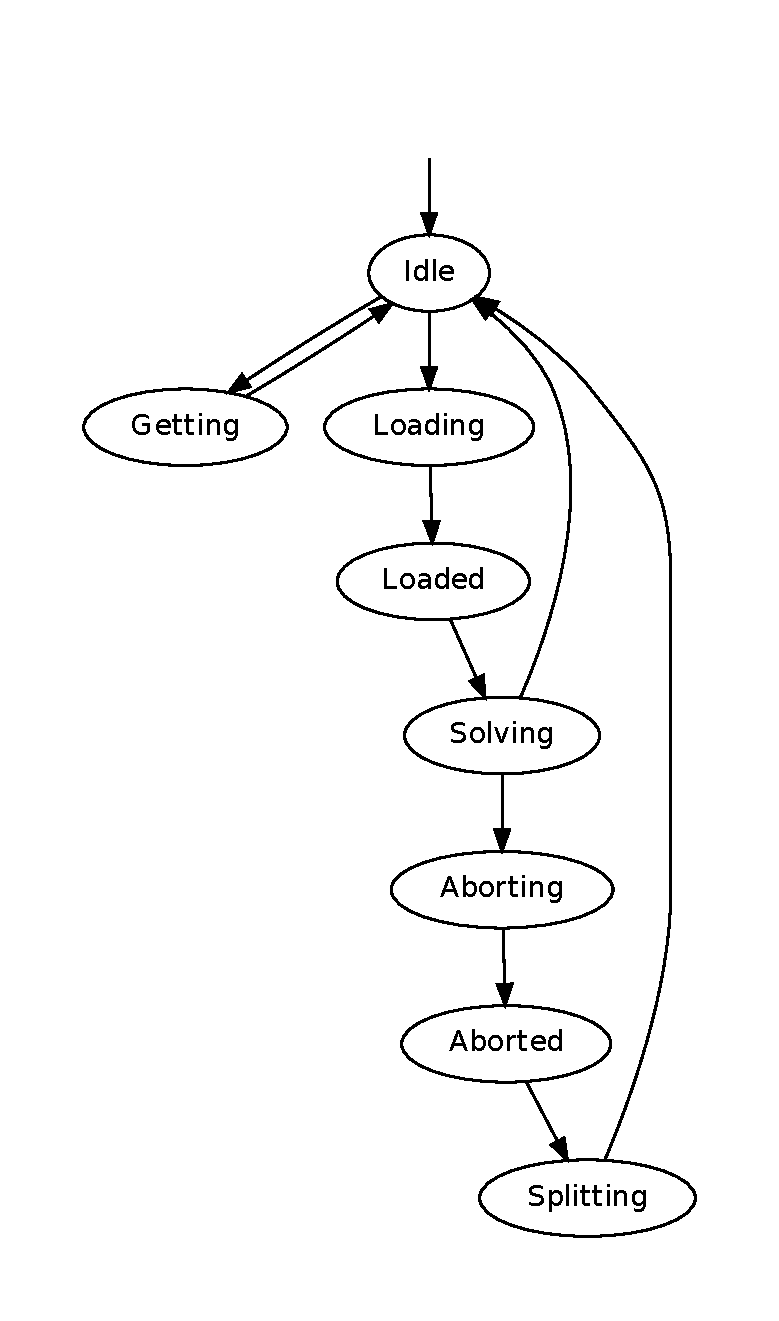
\includegraphics[scale=0.5]{graphs/workerstates}
		\caption{\emph{Workers}}
	\end{subfigure}
	\begin{subfigure}[b]{0.5\textwidth}
		\centering
		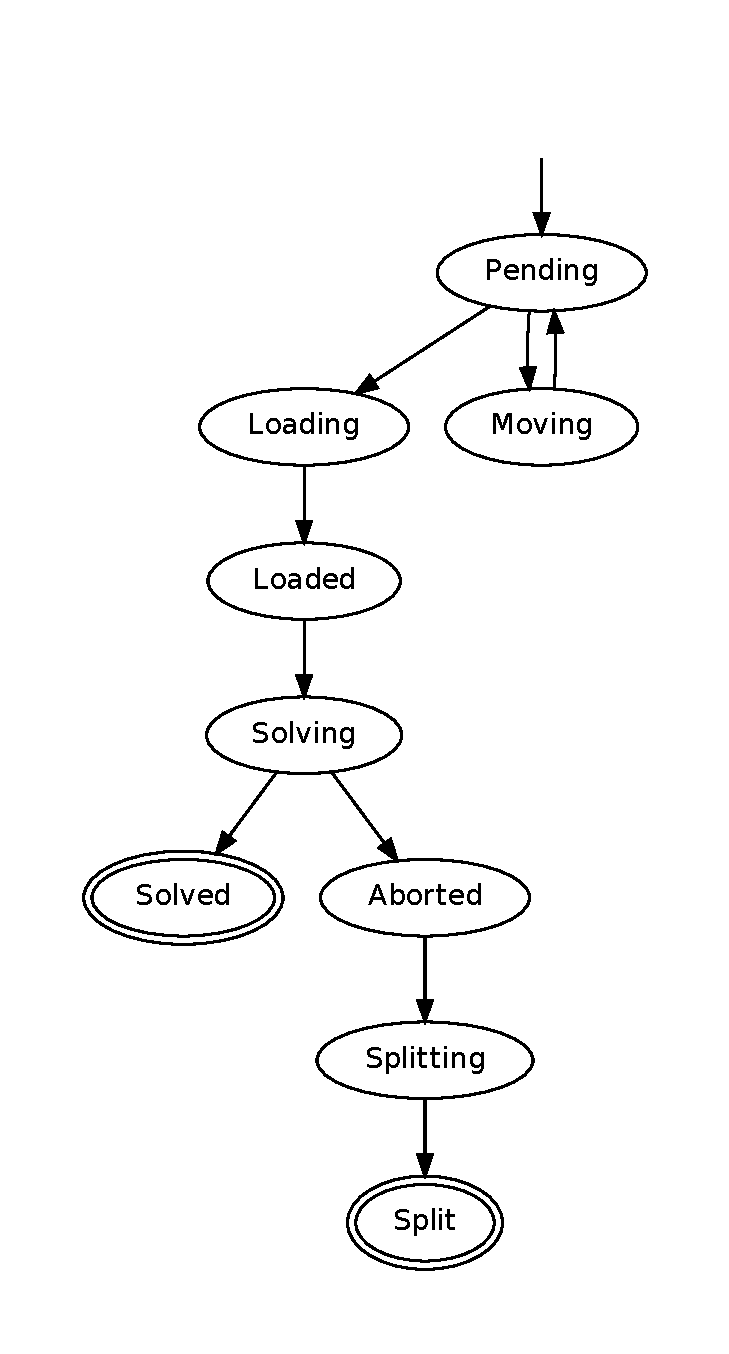
\includegraphics[scale=0.5]{graphs/taskstates}
		\caption{Tareas}
	\end{subfigure}
	\caption{Diagramas de estado en el tablero de control}
\end{figure}

\begin{small}
\begin{lstlisting}[language=Python,caption=Interfaz Strategy]
class Strategy(object):
	def register_globalstate(self, globalstate)
	def register_socket(self, commandsocket)
	def on_init(self, worker)
	def on_createroot(self, worker, task)
	def on_init_finished(self, nworkers)
	def on_getfile(self, worker, task)
	def on_file(self, worker, task)
	def on_load(self, worker, task)
	def on_unsat(self, worker, task)
	def on_sat(self, worker, task, modelstr)
	def on_abort(self, worker, task)
	def on_split_newtask(self, worker, newtask)
	def on_split_finished(self, worker, parenttask, nchildren)
	def on_shutdown(self)
\end{lstlisting}
\end{small}

\subsubsection{Nuestra estrategia}

\subsection{Decisiones que vale la pena seguir investigando}

\section{Resultados experimentales}

%!TEX root = tesis.tex
\chapter{Aprendizaje en un \ssolver paralelo y distribuido}
\label{aprendizaje-pardist}

En el Cap.~\ref{ssolver-pardist} vimos que el enfoque de distribución aplicado
consigue disminuir el tiempo necesario para resolver una serie de problemas de
tamaño considerable. Al mismo tiempo observamos que existen casos en los que
la eficiencia --entendida como cuánto ganamos por cada unidad de \hard
agregada al cómputo de un problema-- resulta pobre. Planteamos como hipótesis
que esta situación se debe, en gran medida, a una importante cantidad de
retrabajo que se produce como consecuencia del particionado de un problema en
diversos subproblemas. 

La existencia de retrabajo se evidencia en que si bien al partir un problema
en subproblemas, el subproblema más grande suele ser más chico que el padre,
la suma del tiempo requerido para resolver todos los subproblemas hijos es
considerablemente mayor que el tiempo requerido para resolver el problema
padre. Debido al esquema de particionado recursivo, este incremento en el
tiempo total de cómputo requerido para resolver un problema se vuelve
sustancial.

En el presente capítulo desarrollaremos un mecanismo de reutilización del
conocimiento adquirido durante la ejecución de cada subproblema. Este
mecanismo persigue dos objetivos principales: verificar la hipótesis planteada
y, de ser posible,  disminuir los tiempos requeridos para resolver un problema
aumentando la eficiencia de la herramienta.

\section{Justificación del enfoque}

El enfoque de particionamiento recursivo, basado en \emph{guiding paths}, que
hemos adoptado para la construcción de la herramienta también influye en la
elección de un mecanismo adecuado para compartir información de cláusulas
aprendidas. 

\newcommand{\roottask}{\ensuremath{<\varphi_R, \emptyset>}\xspace}
\newcommand{\task}{\ensuremath{<\varphi, \emptyset>}\xspace}
\newcommand{\nonemptytask}{\ensuremath{<\varphi, C>}\xspace}

Consideremos ahora que un problema no es ya únicamente una fórmula $\varphi$
sino una tupla $<\varphi, C>$ donde $C$ es un conjunto de cláusulas tales que
$(\forall v) (v \models \varphi \Longleftrightarrow v \models \varphi
\bigwedge C)$ llamado conjunto de cláusulas aprendidas. En este contexto el
problema original es la tupla \roottask donde $\varphi_R$ denota la fórmula
original que se desea verificar. En este modelo, al partir un problema \task
levantando (por ejemplo) la variable $u$ obtenemos dos nuevos subproblemas
$<\varphi_u, \emptyset>$ y $<\varphi_{-u}, \emptyset>$. 

Notemos entonces que dado un problema \nonemptytask podemos generar los
subproblemas que resultan de levantar la variable $u$ como sigue:
$t_u=<\varphi_u, C_u>$ y $t_{-u}=<\varphi_{-u}, C_{-u}>$ (donde $C_u$ es el
conjunto de cláusulas que resulta de reemplazar las apariciones de la variable
$u$ por el valor $1$ en el conjunto $C$ y $C_{-u}$ es el resultado de
reemplazar las apariciones de la variable $u$ por el valor $0$) sin alterar la
corrección de la herramienta. Esto se debe a que si $v \models \varphi_u$
entonces $v\cup\{u\leftarrow1\} \models \varphi$ y por lo tanto
$v\cup\{u\leftarrow1\} \models \varphi \bigwedge C$ de lo que se deduce que $v
\models \varphi_u \bigwedge C_u$. Lo mismo vale para el caso $\varphi_{-u}$.

Más aún, lo antedicho vale también para cualquier subconjunto de $C$. Esto
induce una manera \emph{natural} de reutilización de las cláusulas aprendidas
que llamaremos \emph{herencia}. Este mecanismo consiste en que, al generar
nuevos subproblemas a partir de un problema padre \nonemptytask, los
subproblemas hijos son generados con un subconjunto de $C$ como conjunto de
cláusulas aprendidas. Llamaremos \emph{criterio} a cada forma distinta de
obtener un subconjunto a partir de un conjunto de cláusulas $C$.


\subsubsection{Consideraciones de escalabilidad}

Más allá de la naturalidad del enfoque inducido por el esquema de
particionado, nos interesa también evitar cualquier método que introduzca
nuevos cuellos de botella en la arquitectura. Por ejemplo, no sería aceptable
la incorporación de una gran base de datos centralizada en la que todos los
\ws almacenen las cláusulas que van aprendiendo y que todos los \ws deban
consultar.

Tampoco sería aceptable un grafo completo de comunicación permanente para
lograr ese mismo fin, es decir, hacer que cada \w le comunique (o consulte) a
todos los demás las cláusulas que va(n) aprendiendo.


\subsubsection{Independencia del \ssolver particular utilizado}

Por otro lado, como ya hemos señalado en el Cap.~\ref{ssolver-pardist}, nos
interesa que el \ssolver secuencial que utiliza cada uno de los \ws sea fácil
de actualizar y/o de reemplazar por otro componente \ots similar. Si bien
suelen ser necesarios algunos cambios para lograr que un \ssolver permita la
inyección \emph{inicial} de cláusulas aprendidas (en lugar de comenzar sin
ninguna), por lo general tales cambios se reducen a cuestiones de interfaz y
no revisten mayor dificultad.

Es más ambicioso, en cambio, pretender poder inyectar nuevas cláusulas
aprendidas en cualquier momento \emph{durante} el proceso de búsqueda. Para
ello habría que introducir modificaciones mucho más fuertemente acopladas a la
versión particular de \ssolver en uso, sus algoritmos, estructuras de datos e
invariantes particulares.

\

Es por estos factores que optamos por implementar un esquema de reutilización
de cláusulas aprendidas basado en herencia. En esencia el esquema funciona de
acuerdo a lo detallado al comienzo de esta sección. En particular, a la hora
de partir un problema en nuevos subproblemas un \emph{criterio} es aplicado al
conjunto de cláusulas aprendidas que el problema padre poseía al momento de
ser abortado. De esta manera se generan los subconjuntos de cláusulas
aprendidas que los subproblemas hijos deberán incorporar antes de comenzar el
análisis. Cabe destacar que si bien la herramienta permite seleccionar un
nuevo criterio de aprendizaje cada vez que un problema es partido, en la
evaluación realizada no se utilizó esta característica sino que se mantuvo un
mismo criterio para toda la corrida.


\subsubsection{Sobre los criterios}

En principio podríamos preguntarnos de dónde surge la necesidad de tener
criterios para la herencia de cláusulas aprendidas. O lo que es lo mismo, por
qué no heredar todas las cláusulas aprendidas del padre. Existen varias
razones que motivan la necesidad de introducir criterios de selección de
cláusulas.

En primer lugar la incorporación de cláusulas aprendidas a un problema
incrementa la cantidad de cláusulas sobre las que es necesario propagar las
decisiones. Esto provoca una ralentización del proceso de propagación que
puede resultar en una disminución del rendimiento del \ssolver secuencial. La
información experimental presentada en diversos artículos muestra que,
incrementar en demasía la base de datos de cláusulas aprendidas en un \ssolver
secuencial, se torna contraproducente. Es por esto que los \ssolvers
secuenciales cuentan con políticas de recorte de dicha base de datos y que,
por lo general, estas políticas son bastante agresivas.

Otro factor que aboga en contra de mantener la totalidad de las cláusulas
aprendidas por el padre es el hecho de que los subproblemas generados suelen
ser más chicos que el padre. Incluso es bastante común que una buena
proporción de los subproblemas generados al partir un problema padre sean
considerablemente más chicos. En todos estos casos la incorporación de una
conjunto de cláusulas aprendidas extremadamente grande, resultará
inmediatamente contraproducente debido a lo expuesto en el párrafo anterior.

El último motivo para la introducción de criterios de selección es que el
conjunto de cláusulas aprendidas de un problema es potencialmente muy grande.
Por otro lado, los subproblemas generados no son resueltos inmediatamente sino
que pasan a formar parte de la cola de tareas pendientes. Es decir que,
heredar la totalidad de las cláusulas aprendidas del problema padre en cada
uno de los subproblemas hijos, nos obligaría a pagar un alto costo debido a la
escritura y posterior lectura --hacia y desde memoria secundaria-- de cada
unos de estos conjuntos (potencialmente muy grandes) más el costo de la
posible transmisión por medio de la red. Esto atentaría directamente contra el
desempeño de nuestra herramienta, incrementando en demasía los costos
\emph{fijos} asociados al enfoque.

% Que cada hijo herede TODAS las cláusulas aprendidas por su padre probablemente sea demasiado / contraproducente:
% \begin{itemize}
% \item Por algo los solvers secuenciales van purgando: es sabido que zarparse no es bueno.
% \item OK, el padre sí llegó a todo eso, pero por algo los solvers secuenciales van subiendo de a poco el máximo de aprendidas: es sabido que zarparse desde el primer momento no es buena idea. Y estamos suponiendo que los subproblemas serán más chicos/fáciles que su problema padre.
% \item Y además, la herencia no es inmediata sino mediata. Jugarse a heredar todo implica jugarse a pagar el precio de bajar todo eso a disco, guardar todo eso en storage/pending, leer todo eso de disco, etc. Bocha overhead.
% \end{itemize}

% Por lo tanto vamos a necesitar criterios de selección, subconjunto, etc.


\section{Prueba de concepto}

Con el objetivo de evaluar la pertinencia y viabilidad del enfoque propuesto
para el aprendizaje, llevamos a cabo una prueba de concepto. La misma
consistió en la ejecución de distintos problemas realizando una única
partición y aplicando distintos criterios de selección de cláusulas aprendidas
y comparando los tiempos obtenidos. Para ello cada problema fue ejecutado
durante 60 segundos y luego partido levantando 5 variables para obtener 32
subproblemas. Cada uno de los subproblemas fue ejecutado hasta su
finalización. Dado que, como ya mencionamos, la elección de variables a
levantar influye fuertemente en la distribución de dificultades de los
subproblemas resultantes, cada criterio fue testeado utilizando 10 secuencias
de variables distintas generadas pseudoaleatoriamente. Luego se compararon
tanto los tiempos totales de cómputo invertidos en resolver el problema, como
el tiempo del camino crítico (determinado por el subproblema que más tiempo
tomó).


\subsubsection{Resultados obtenidos}

A continuación presentamos los resultados obtenidos en la realización de la
prueba de concepto. Las Fig.~\ref{perchap8}~a~\ref{perchasound8}  se organizan
de la siguiente manera. Cada figura corresponde a la ejecución de distintos
criterios de selección de cláusulas para un problema particular. Cada par de
columnas denotadas con un número decimal corresponde a los resultados
obtenidos con uno de los órdenes pseudoaleatorios. La columna de la izquierda
de cada par de columnas indica el tiempo en segundos requerido para resolver
el camino crítico. Mientras tanto la columna de la derecha indica la sumatoria
del total de tiempos requerido para resolver todos los subproblemas. A su vez,
el último par de columnas de cada figura, denotado con la leyenda ``AVERAGE''
contiene los promedios de los tiempos obtenidos.

No nos interesaba en esta etapa evaluar cuál o cuáles de los criterios eran
mejores. Por lo tanto obviamos la denominación de los mismos en esta
presentación. Sin embargo es importante aclarar que la última fila contiene
los tiempos obtenidos para el criterio nulo, es decir aquel criterio que
devuelve siempre el conjunto vacío.

El coloreo de las tablas se realizó utilizando una escala desde el color
amarillo hacia el rojo para aquellos criterios que requirieron más tiempo que
el criterio nulo, mientras que se usó una escala del amarillo hacia el verde
para los que requirieron menos tiempo. La escala hacia el color rojo se saturó
en dos veces el tiempo requerido por el criterio nulo mientras que la escala
hacia el verde se saturó en $0.5$ veces el tiempo requerido por el criterio nulo.

\begin{figure}
	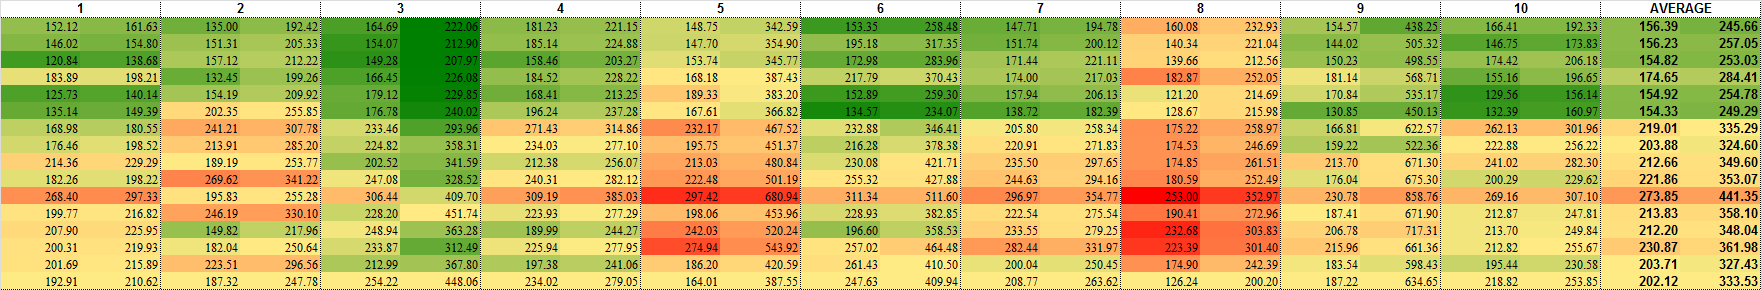
\includegraphics[width=\textwidth]{resultados/p8_percha.png}
	\caption{Routing \emph{scope} 8}
	\label{perchap8}
\end{figure}

\begin{figure}
	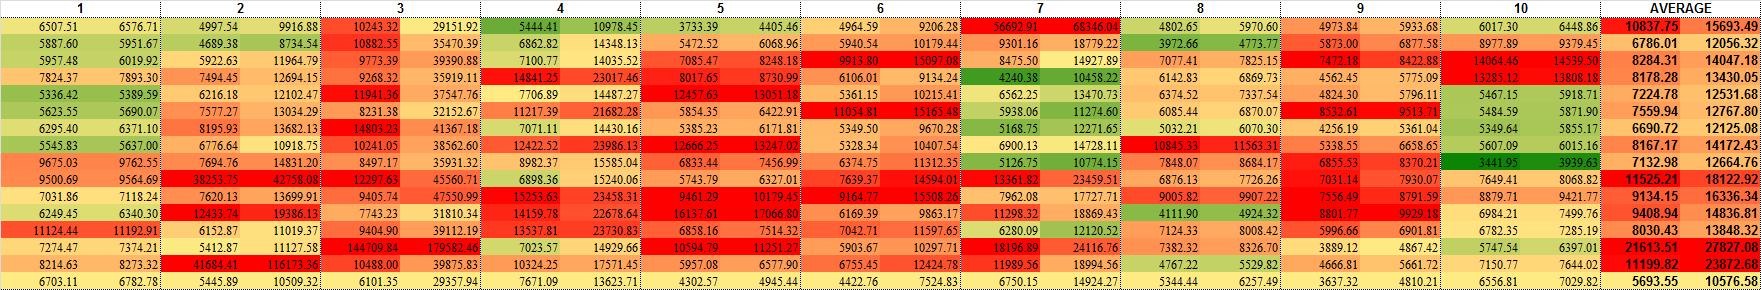
\includegraphics[width=\textwidth]{resultados/p9_percha.png}
	\caption{Routing \emph{scope} 9}
\end{figure}

\begin{figure}
	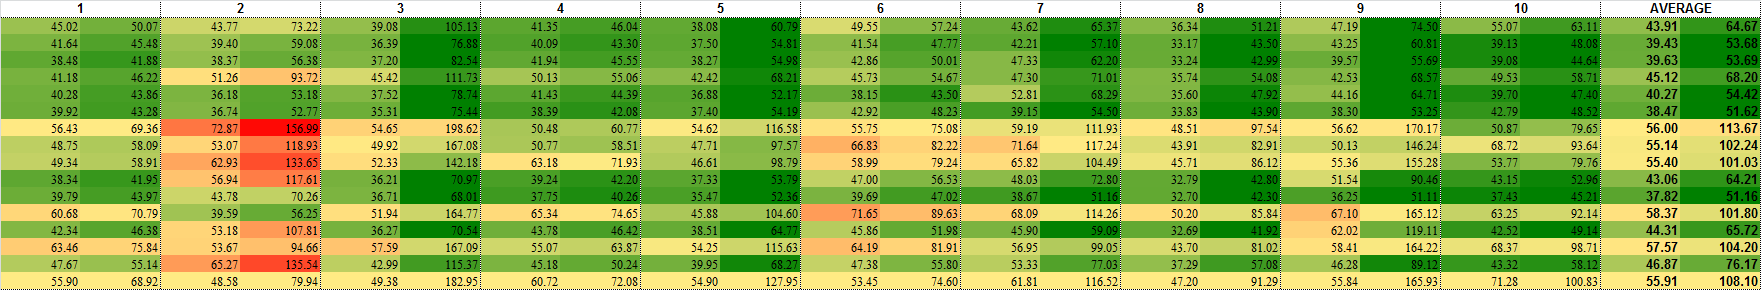
\includegraphics[width=\textwidth]{resultados/k9_percha.png}
	\caption{Closure \emph{scope} 9}
\end{figure}

\begin{figure}
	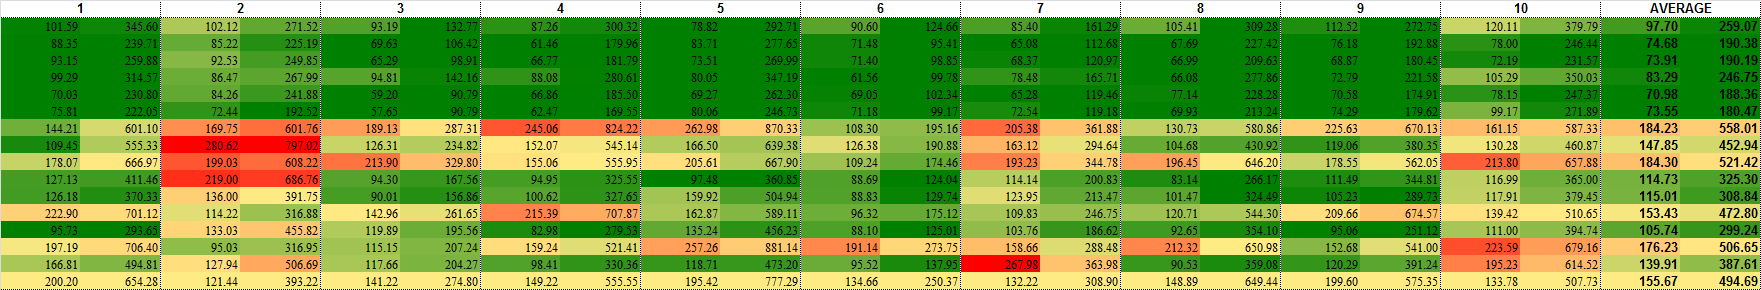
\includegraphics[width=\textwidth]{resultados/k10_percha.png}
	\caption{Closure \emph{scope} 10}
\end{figure}

\begin{figure}
	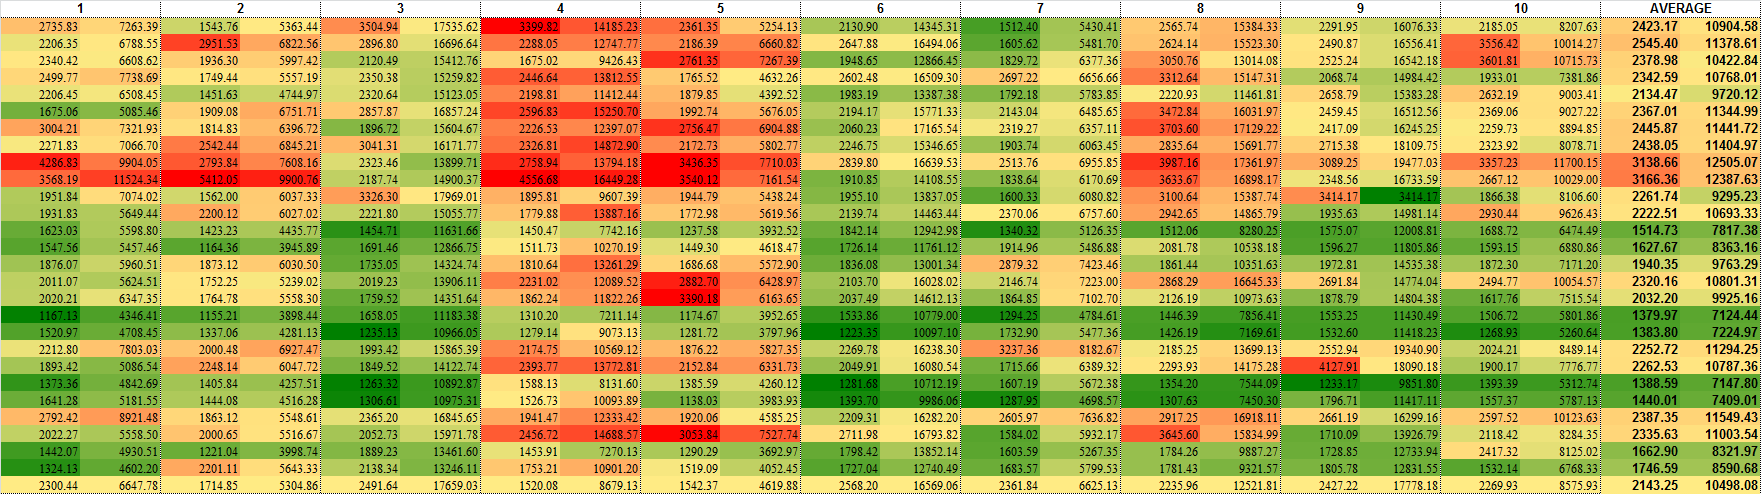
\includegraphics[width=\textwidth]{resultados/soundness8_percha.png}
	\caption{Soundness2 \emph{scope} 8}
	\label{perchasound8}
\end{figure}

Como puede observarse en las figuras, los resultados obtenidos varían
fuertemente de uno a otro problema y en función de cada elección particular de
variables. Además, los resultados no podrían ser del todo concluyentes en
tanto constituyen una aproximación de orden 1 al enfoque \emph{divide-and-
conquer}: en esta prueba de concepto, el problema no se parte recursivamente
sino una única vez en subproblemas.

Más allá de estas limitaciones, cabe observar que en algunos casos varios de
los criterios reportan ganancias considerables. Aún más importante es el hecho
de que para la mayoría de los problemas hay al menos un criterio que reporta
resultados positivos. Interpretamos esto como evidencia suficientemente
alentadora como para embarcarnos en una evaluación más realista de la técnica
en el marco de nuestra herramienta distribuida.

\section{Resultados experimentales}

En esta sección mostraremos los resultados experimentales obtenidos a partir
de la implementación de la herencia de cláusulas aprendidas.

Comenzaremos por definir los criterios de selección de cláusulas utilizados.
Cabe aclarar que de aquí en más se considerará que una cláusula aprendida
contiene al menos $2$ literales. Llamaremos \emph{hechos} a las cláusulas de
tamaño $1$.

\subsection{Criterios de selección de cláusulas}

Se probaron tres tipos de criterios:

\begin{itemize}
	\item Por tamaño: Este criterio refiere a la cantidad de literales intervinientes en una cláusula. La motivación de este criterio surge de la observación de que, cuanto más pequeña sea una cláusula, mayor será la porción del árbol de búsqueda que recorte. Recordemos que, en el contexto de nuestro problema, las cláusulas son disyuciones. Por lo tanto una cláusula que contiene $n$ literales nos evita recorrer una $\frac{1}{2^n}$ parte del espacio de búsqueda. Esto se debe a que, de las $2^n$ valuaciones posibles restringidas a los $n$ literales intervinientes, hay una de ellas --en particular aquella que hace que dicha cláusula sea falsa-- que es descartada gracias a la existencia de esta cláusula aprendida. Por lo tanto ninguna valuación que contenga dicha valuación restringida será viable. Por ende, a menor tamaño de cláusula, mayor será el espacio de búsqueda recortado.

	\item Por actividad: En \ref{sec:longactlbd} se explicó a qué nos referimos por actividad de una cláusula. De ello se desprende que la actividad de una cláusula es un indicador de cuántas veces esa cláusula fue (parcialmente) responsable de que ocurra un conflicto. Es de esperar entonces que las cláusulas con mayor actividad sean más relevantes para evitar recorrer ciertas porciones del espacio de de búsqueda.

	\item Por \emph{LBD}: También en \ref{sec:longactlbd} introdujimos la noción de \emph{Literals Block Distance}. Elegimos utilizar esta medida porque se han reportado muy buenos resultados en \ssolvers secuenciales \cite{satchallenge12,satcomp11,satcomp09} utilizando criterios basados en esta medida.
\end{itemize}

\subsubsection{Parámetros}

En el caso de los criterios por tamaño, los mismos se generaron a partir de un
parámetro que indica el máximo tamaño que puede terner una cláusula para ser
admitida en la herencia. En este caso, todas las cláusulas cuyo tamaño sea
menor o igual que el indicado por el parámetro pasarán a formar parte de la
herencia.

Los criterios por \emph{LBD} funcionan de la misma manera que los basados en
tamaño. En este caso las cláusulas admitidas en la herencia serán aquellas
cuyo \emph{LBD} sea menor o igual al correspondiente parámetro.

Los criterios por actividad se generan a partir de tres parámetros. En primer
lugar un parámetro binario que indica si se desean conservar las cláusulas más
activas o las menos activas. En segundo lugar un parámetro que indica qué
porcentaje de las cláusulas aprendidas del padre se desea conservar y por
último un parámetro binario que indica si, además, se deben conservar todas
aquellas cláusulas aprendidas cuyo tamaño sea 2 (cláusulas binarias).

La incorporación de las cláusulas binarias en los criterios por actividad
surge del hecho de que, el \ssolver secuencial utilizado recorta su base de
datos de claúsulas aprendidas de acuerdo a la actividad pero nunca descarta
las cláusulas binarias.

Además de los tipos de criterios mencionados también se implementó la
posibilidad de heredar los \emph{hechos} aprendidos (o \emph{facts}). La
herencia de los \emph{facts} se implementó de manera tal que pudiera tanto ser
combinada con los distintos tipos de criterios como también utilizada de forma
exclusiva como criterio de herencia.




\subsection{Resultados obtenidos}

A continuación presentamos los resultados obtenidos. Los mismos se dividen en
tres aspectos diferentes. 

\subsubsection{Validación de la hipótesis de trabajo}

En la Tabla~\ref{tab:mejorlearning} se presenta la comparación entre los
resultados obtenidos con el \ssolver secuencial, los resultados obtenidos por
nuestra herramienta sin herencia de cláusulas aprendidas y los resultados
obtenidos por nuestra herramienta con herencia de cláusulas aprendidas.

Las primeras siete columnas poseen el exacto mismo significado que en la
Tabla~\ref{tab:resultados}. En la columna ``par. walltime w. inher. best crit.'' consignamos
el mejor tiempo obtenido por nuestra herramienta con algún criterio de
selección de cláusulas aprendidas --incluyendo el criterio nulo--.

La columna ``speedup w. inher. best crit.'' representa la mejoría en el tiempo
percibido obtenida por el mejor criterio. La misma es el resultado de la
divisón $$\frac{\text{seq. walltime}}{\text{par. walltime w. inher. best
crit.}}$$ La columna ``efficiency w. inher. best crit.'' es el resultado de la
división $$\frac{\text{speedup w. inher. best crit.}}{\text{\#\ws}}$$ La
columna ``effic. mult.'' es el resultado de la división
$$\frac{\text{efficiency without inheritance}}{\text{efficiency w. inher. best
crit.}}$$

\begin{sidewaystable}
	\small
	\begin{tabular}{lrrrrrrrrrr}
		\toprule
		problem	&			&	reps.	& 	seq.		&  par. walltime	&	speedup				&	efficiency			& par.	walltime				& speedup 							& efficiency			& eff. \\
				&			&	 		& walltime		&  without 			&	without				&	without				& w. inher.	& w. inher. 	& w. inher.	& mult. \\
				&			&	 		& 				& inheritance 		&	 inheritance		&	 inheritance	 	& best crit.	& best crit. 	& best crit.	&  \\
		\cmidrule(r){1-11}
		Routing	&	8		&		7 	& 308.26		&  60.46		& 5.10x		&	0.08 		& 60.46			&	5.10x	& 0.08		& 1.00 \\
		Routing	&	9		&	6 		& 76168.16		&  407.34		& 	186.99x	&	2.92 		& 387.44		& 196.60x	& 3.07		& 1.05 \\
		Routing	&	$^*$10	&	5 		& $>$1209600.00	&  5046.84		&$>$239.67x	&	$>$3.74 	& 3213.59		&$>$376.40x	& $>$5.88	& 1.57 \\
		\cmidrule(r){1-11}
		Closure	&	11		&	14 		& 749.65		&  291.28		&	2.57x	&	0.04 		& 150.30		&  4.99x	& 0.08		& 1.94 \\
		Closure	&	12		&	5 		& 3983.36		&  1914.45		&	2.08x	&	0.03 		& 266.68		& 14.94x	& 0.23		& 7.35 \\
		Closure	&	13		&  5 		& 16261.35		& 	4362.61		&	3.73x	&	0.06 		& 645.44		& 25.19x	& 0.39		& 6.76 \\
		\cmidrule(r){1-11}
		GC Sound.&	9		&	10 		& 217.31		&  200.85		&	1.08x	&	0.02 		& 168.04		& 1.29x		& 0.02		& 1.20 \\
		GC Sound.&	10		&	7 		&  2855.30		&  1376.89		&	2.07x	&	0.03 		& 592.54		& 4.82x		& 0.08		& 2.32 \\
		\cmidrule(r){1-11}
		GC Compl.	& 8		&	7 		& 180.25		&  61.50		&	2.93x	&	0.05 		& 36.43			& 4.95x		& 0.08		& 1.69 \\
		GC Compl.	& 9	&	5 		& 18643.06		&  1825.60		&	10.21x	&	0.16 		& 390.48		& 47.74x	& 0.75		& 4.68 \\
		\bottomrule
		\\
		\multicolumn{10}{l}{\begin{tiny}$^*$: Se ejecutó por 14 días sin que el \ssolver secuencial consiga un resultado\end{tiny}}
	\end{tabular}
	\caption{Tiempo de ejecución (en segundos) distribuido sin herencia vs. distribuido con herencia de cláusulas aprendidas}
	\label{tab:mejorlearning}
\end{sidewaystable}

En casi todos los casos se obtuvo una disminución en los tiempos de cómputo
con respecto a la versión sin herencia de cláusulas aprendidas. Se observa una
única excepción, el problema Routing con \emph{scope} 8. En este caso el mejor
tiempo fue el obtenido por el criterio nulo. Es decir por la herramienta sin
herencia de cláusulas.

Se observa también una tendencia a que la mejora obtenida por la incorporación
de herencia de cláusulas crezca considerablemente a medida que crece el tamaño
del problema.

\subsubsection{Promedios por cada criterio}

En la Tabla~\ref{tab:rescriterios} mostramos los resultados obtenidos para
cada criterio. La columna ``worst speedup (x)'' consigna el peor desempeño
promedio obtenido por el criterio correspondiente para un problema. La columna
``best speedup (x)'' consigna el mejor desempeño promedio obtenido para un
problema.

Por último, la columna ``avg speedup (x)'' consigna el desempeño promedio
obtenido por los criterios considerando todos los problemas. Este valor se
calculó comparando la suma de los tiempos promedio de todos los problemas
--sin herencia de cláusulas aprendidas-- contra la suma de los tiempos
promedio de todos los problemas utilizando el criterio correspondiente. Hay
que tener en cuenta entonces que las mejoras obtenidas en problemas más
grandes pesarán más que las mejoras obtenidas en problemas más chicos.

Es importante señalar que en esta tabla no aparecen absolutamente todos los
criterios. El motivo de esto es que no todos los criterios pudieron ser
probados con todos los problemas. Como se verá más adelante, algunos criterios
resultaron claramente perjudiciales. Por lo tanto, dichos criterios no fueron
probados con los problemas más grandes --Routing \emph{scope} 10, Closure
\emph{scope} 13, etc--.

En cada columna se señalaron con color verde los mejores resultados obtenidos
en dicha columna y con color rojo los peores resultados obtenidos.

\begin{table}
	\small
	\begin{tabular}{lrrr}
		\toprule
					&	worst 		&	best		&	avg \\
		criteria	&	speedup (x)	&	speedup (x)	&	speedup (x) \\
		\cmidrule(r){1-4}
		lbdle2.+facts	&	0.68	&	4.91	&	1.97 \\
		lbdle2.-facts	&	0.71	&	3.84	&	1.24 \\
		lbdle3.+facts	&	0.78	&	5.16	&	1.41 \\
		lbdle3.-facts	&	0.75	&	5.71	&	1.69 \\
		lbdle4.+facts	&	0.64	&	6.80	&	1.68 \\
		lbdle4.-facts	&	0.79	&	5.83	&	1.83 \\
		lbdle5.+facts	&	0.69	&	6.74	&	1.64 \\
		lbdle5.-facts	&	0.77	&	5.25	&	2.14 \\
		lbdle6.+facts	&	0.76	&	5.79	&	1.95 \\
		lbdle6.-facts	&	0.70	&	6.08	&	1.94 \\
		\cmidrule(r){1-4}
		onlyfacts	&	\cellcolor{green}0.84	&	3.23	&	1.45 \\
		\cmidrule(r){1-4}
		perc=0.01.+facts.+binary.+active	&	\cellcolor{red}0.55	&	3.83	&	2.12 \\
		perc=0.01.+facts.+binary.-active	&	0.77	&	3.78	&	1.92 \\
		perc=0.01.+facts.-binary.+active	&	0.64	&	3.64	&	\cellcolor{red}1.19 \\
		perc=0.01.+facts.-binary.-active	&	0.65	&	3.50	&	1.39 \\
		perc=0.01.-facts.+binary.+active	&	0.74	&	2.73	&	1.91 \\
		perc=0.01.-facts.+binary.-active	&	0.69	&	2.38	&	1.30 \\
		perc=0.01.-facts.-binary.+active	&	0.74	&	\cellcolor{red}1.68	&	1.22 \\
		perc=0.01.-facts.-binary.-active	&	0.71	&	2.22	&	1.22 \\
		\cmidrule(r){1-4}
		sizele2.+facts	&	0.75	&	3.50	&	1.57 \\
		sizele2.-facts	&	0.81	&	3.32	&	\cellcolor{red}1.19 \\
		sizele3.+facts	&	\cellcolor{red}0.55	&	5.40	&	1.63 \\
		sizele3.-facts	&	0.75	&	3.87	&	1.39 \\
		sizele4.+facts	&	0.74	&	6.24	&	1.91 \\
		sizele4.-facts	&	0.72	&	4.21	&	1.81 \\
		sizele5.+facts	&	0.64	&	6.14	&	1.92 \\
		sizele5.-facts	&	0.58	&	\cellcolor{green}7.18	&	1.90 \\
		sizele6.+facts	&	0.72	&	5.08	&	2.17 \\
		sizele6.-facts	&	0.79	&	5.69	&	\cellcolor{green}2.61 \\
		\bottomrule
	\end{tabular}
	\caption{Peor \emph{speedup} para un problema, mejor \emph{speedup} para un problema y \emph{speedup} promedio obtenido por cada uno de los criterios probados}
	\label{tab:rescriterios}
\end{table}

En estos resultados se observa que no hubo ningún criterio que sea siempre
mejor o igual que el criterio nulo. A su vez, el criterio que consiste en
heredar únicamente los hechos aprendidos --cláusulas de tamaño 1-- resultó ser
el que mejor ``worst speedup'' obtuvo. Es decir que este criterio resultó ser
el más seguro en tanto que en el peor caso producirá un resultado un 19\% peor
que si no hubiéramos utilizado ningún tipo de herencia.

También se puede ver que hay más de un criterio que presenta una mejora
promedio (es decir sobre todos los problemas) superior a $2x$ siendo el máximo
obtenido $2.61x$. Es decir que de haber utilizado dicho criterio habríamos
tenido que invertir el 38\% del tiempo que tomó resolver los mismos problemas
sin herencia de cláusulas.

Por último observamos que existen criterios que presentan mucha varianza. Por
ejemplo, el criterio que obtuvo el mejor \emph{speedup} ($7.18x$) para algún
problema obtuvo como peor \emph{speedup} un valor de $0.58x$ muy cercano al
peor de todos.

\subsubsection{Comportamiento de la herencia para \emph{scopes} crecientes}

A continuación presentamos la comparación de los resultados obtenidos por los
distintos criterios para diferentes \emph{scopes} de un mismo problema. Las
Figuras~\ref{res:learnscopespamela}~a~\ref{res:learnscopescompleteness}
presentan los resultados de la siguiente manera. 

La primer fila (coloreada siempre de amarillo) representa el resultado
obtenido por el criterio nulo. Las filas subsiguientes representan los
resultados obtenidos por el criterio indicado a la izquierda. El color que
posee cada celda representa la comparación entre el resultado obtenido por ese
criterio y el resultado obtenido por el criterio nulo para el correspondiente
\emph{scope} de acuerdo a la escala indicada a la derecha de la figura. Así el
coloreo hacia el verde indica una mejora respecto del criterio nulo mientras
que el coloreo hacia el rojo representa una peor desempeño con respecto al
mismo criterio.

En el eje horizontal se ubican los distintos \emph{scopes} probados de manera
creciente. Vale aclarar que el color gris indica la ausencia de resultados
para dicha combinación de \emph{scope} y criterio.

Corresponde aclarar también que, tal como se observa, no todos los criterios
fueron probados para el problema ``GC Completeness''. \todo{Aclarar por qué? ¿Cómo?}

\begin{figure}
	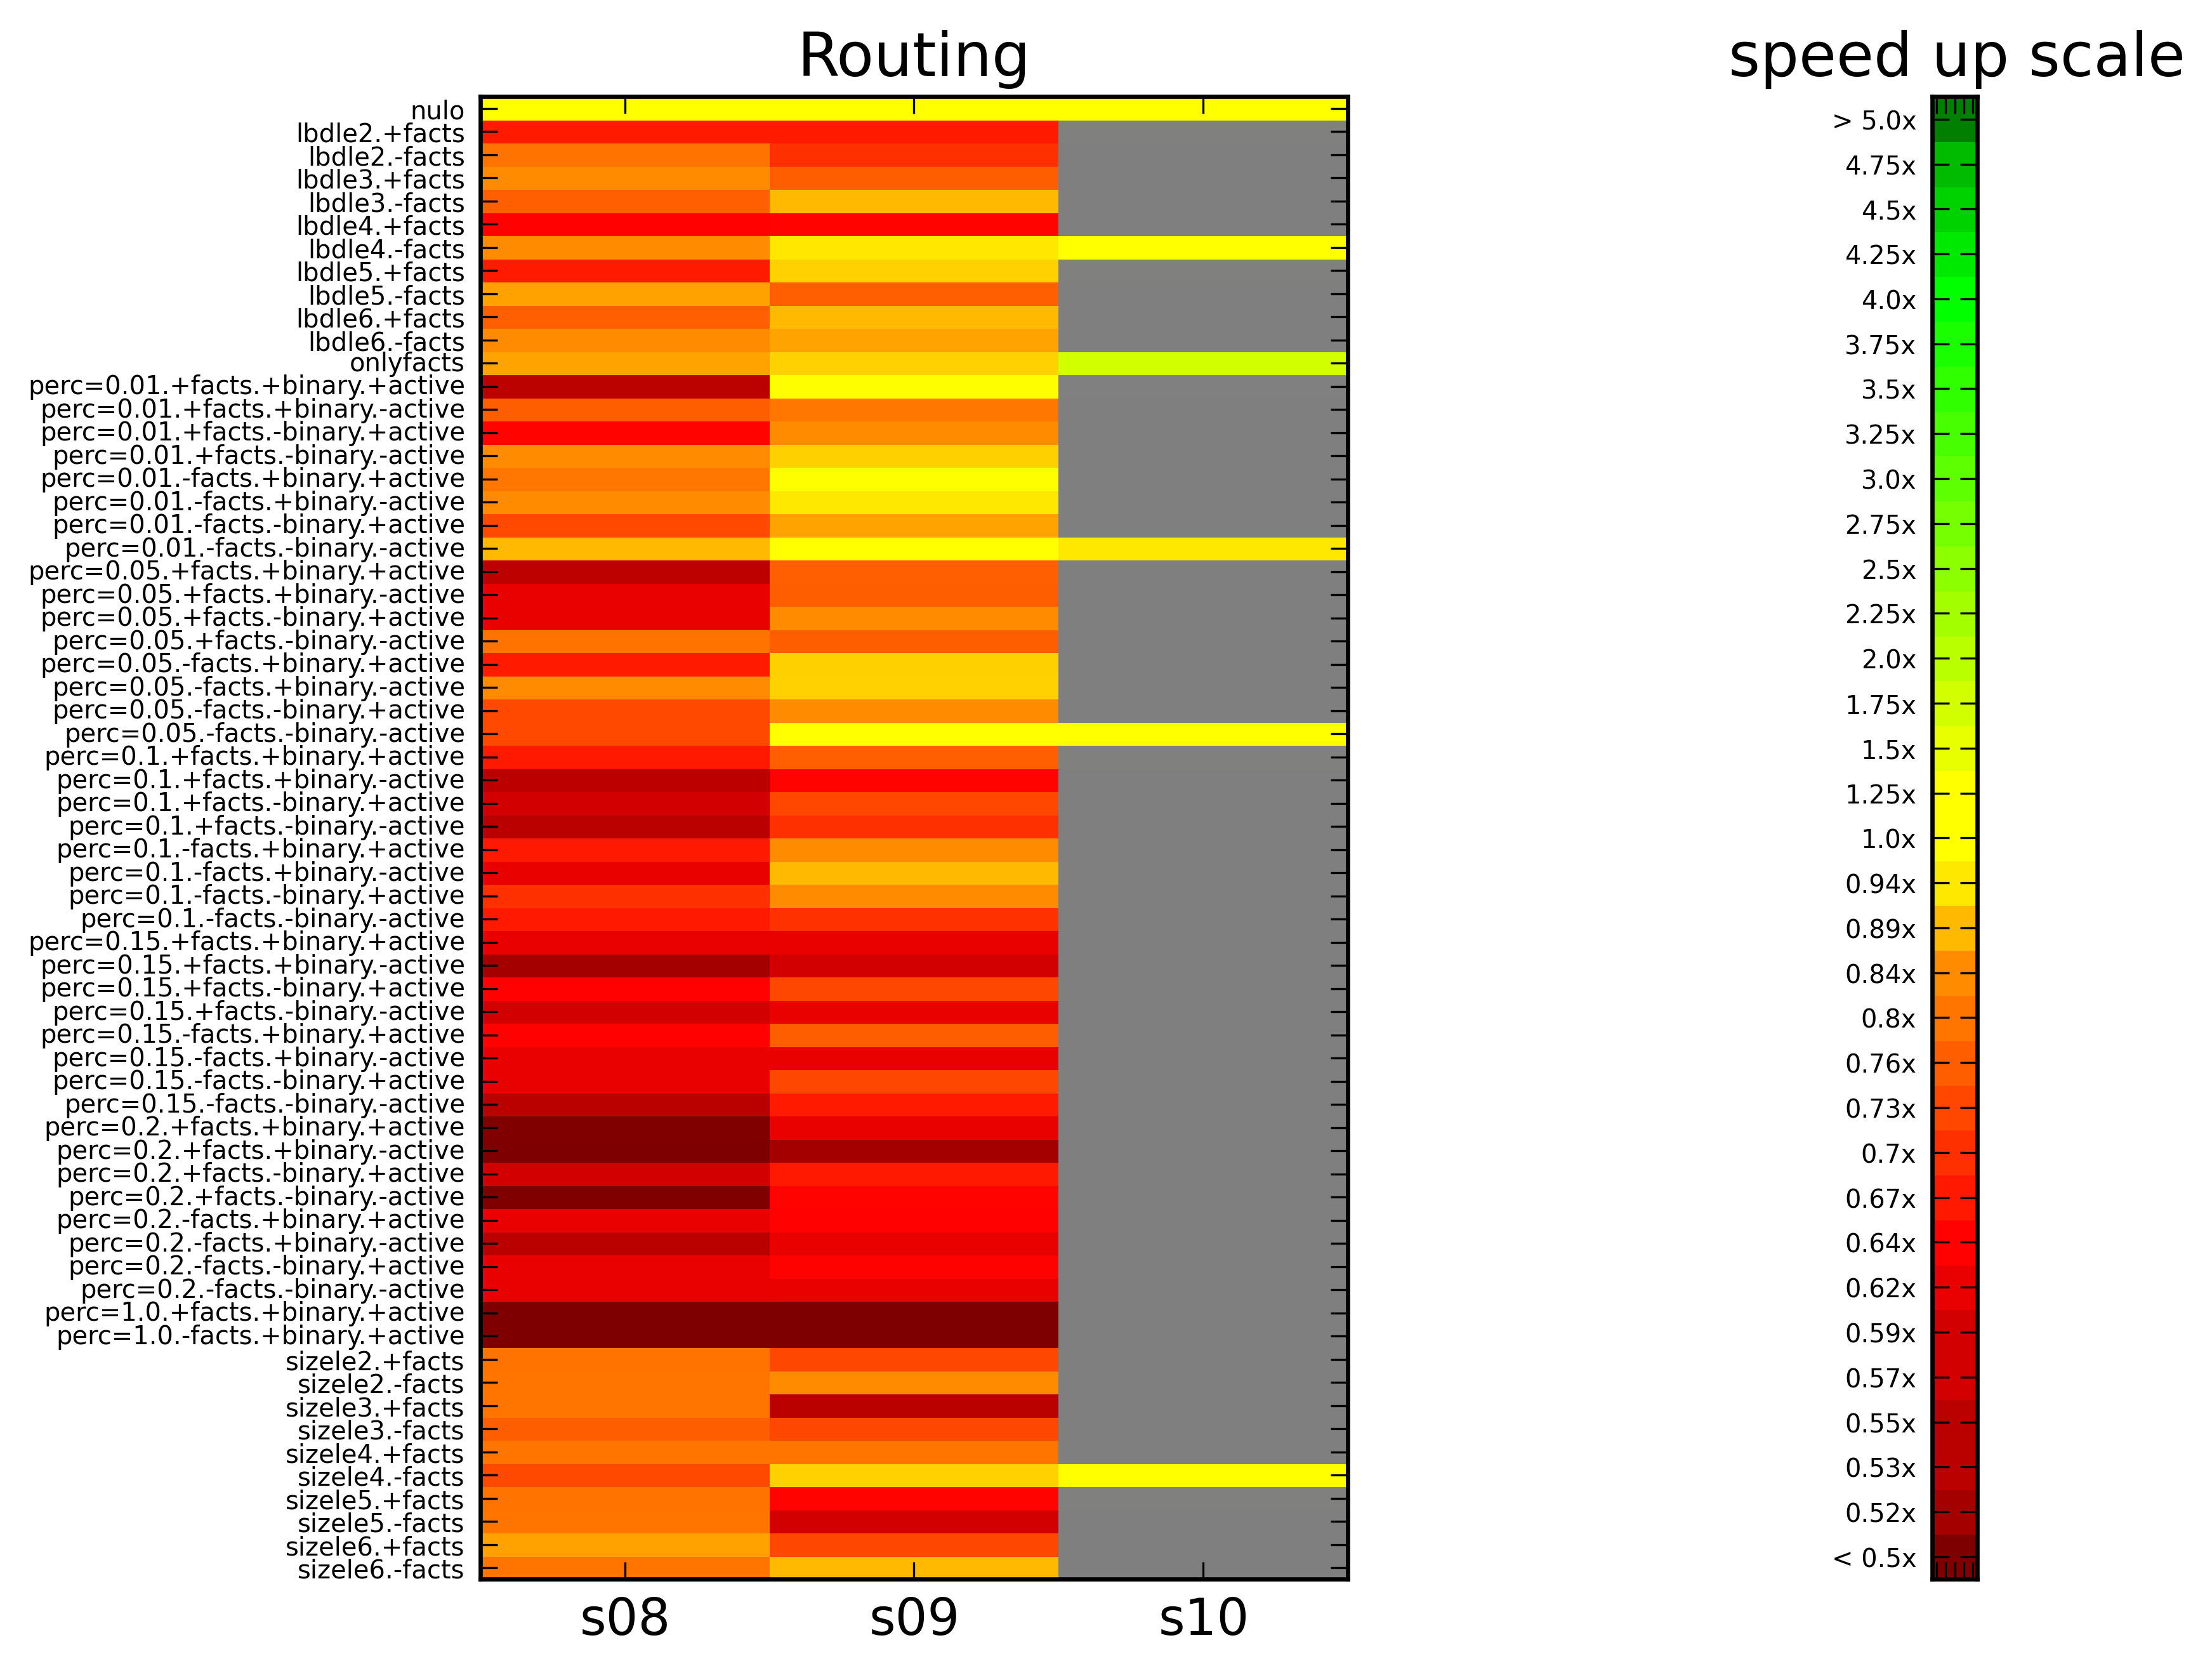
\includegraphics[width=\textwidth]{resultados/losp_heat.png}
	\caption{Comparación de criterios de herencia para distintos \emph{scopes} para el problema Routing}
	\label{res:learnscopespamela}
\end{figure}

\begin{figure}
	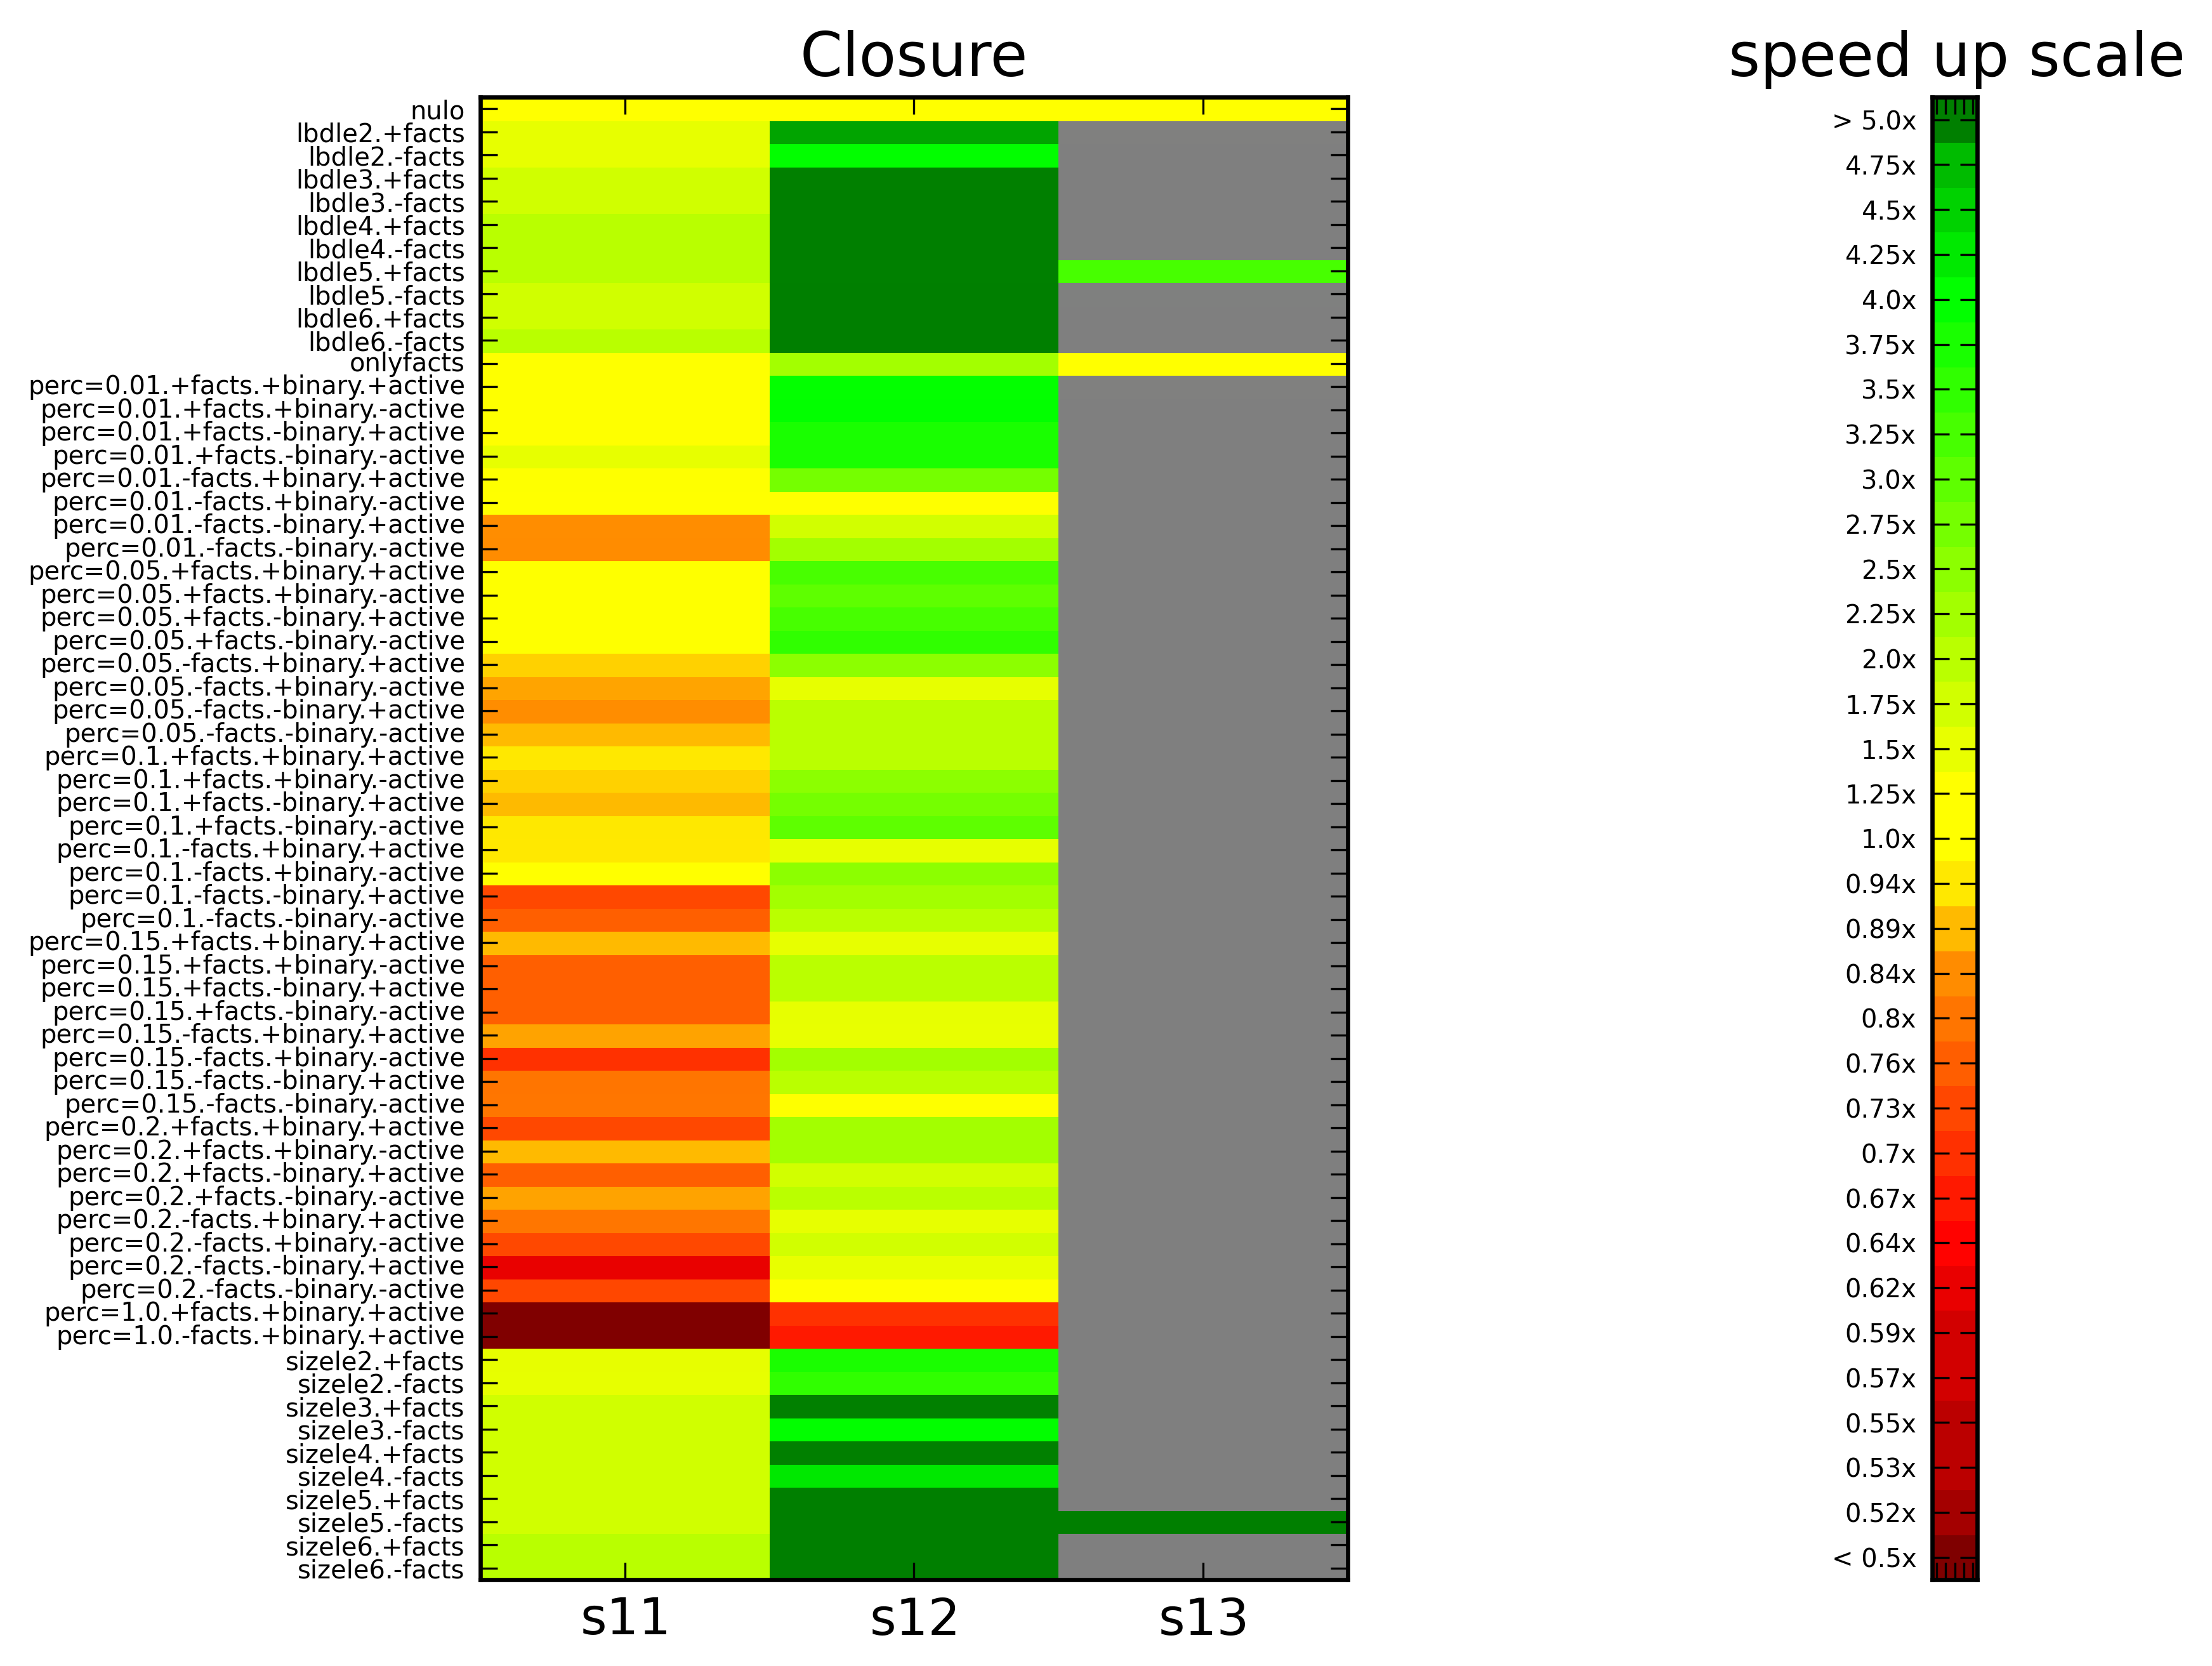
\includegraphics[width=\textwidth]{resultados/losk_heat.png}
	\caption{Comparación de criterios de herencia para distintos \emph{scopes} para el problema Closure}
	\label{res:learnscopesclosure}
\end{figure}

\begin{figure}
	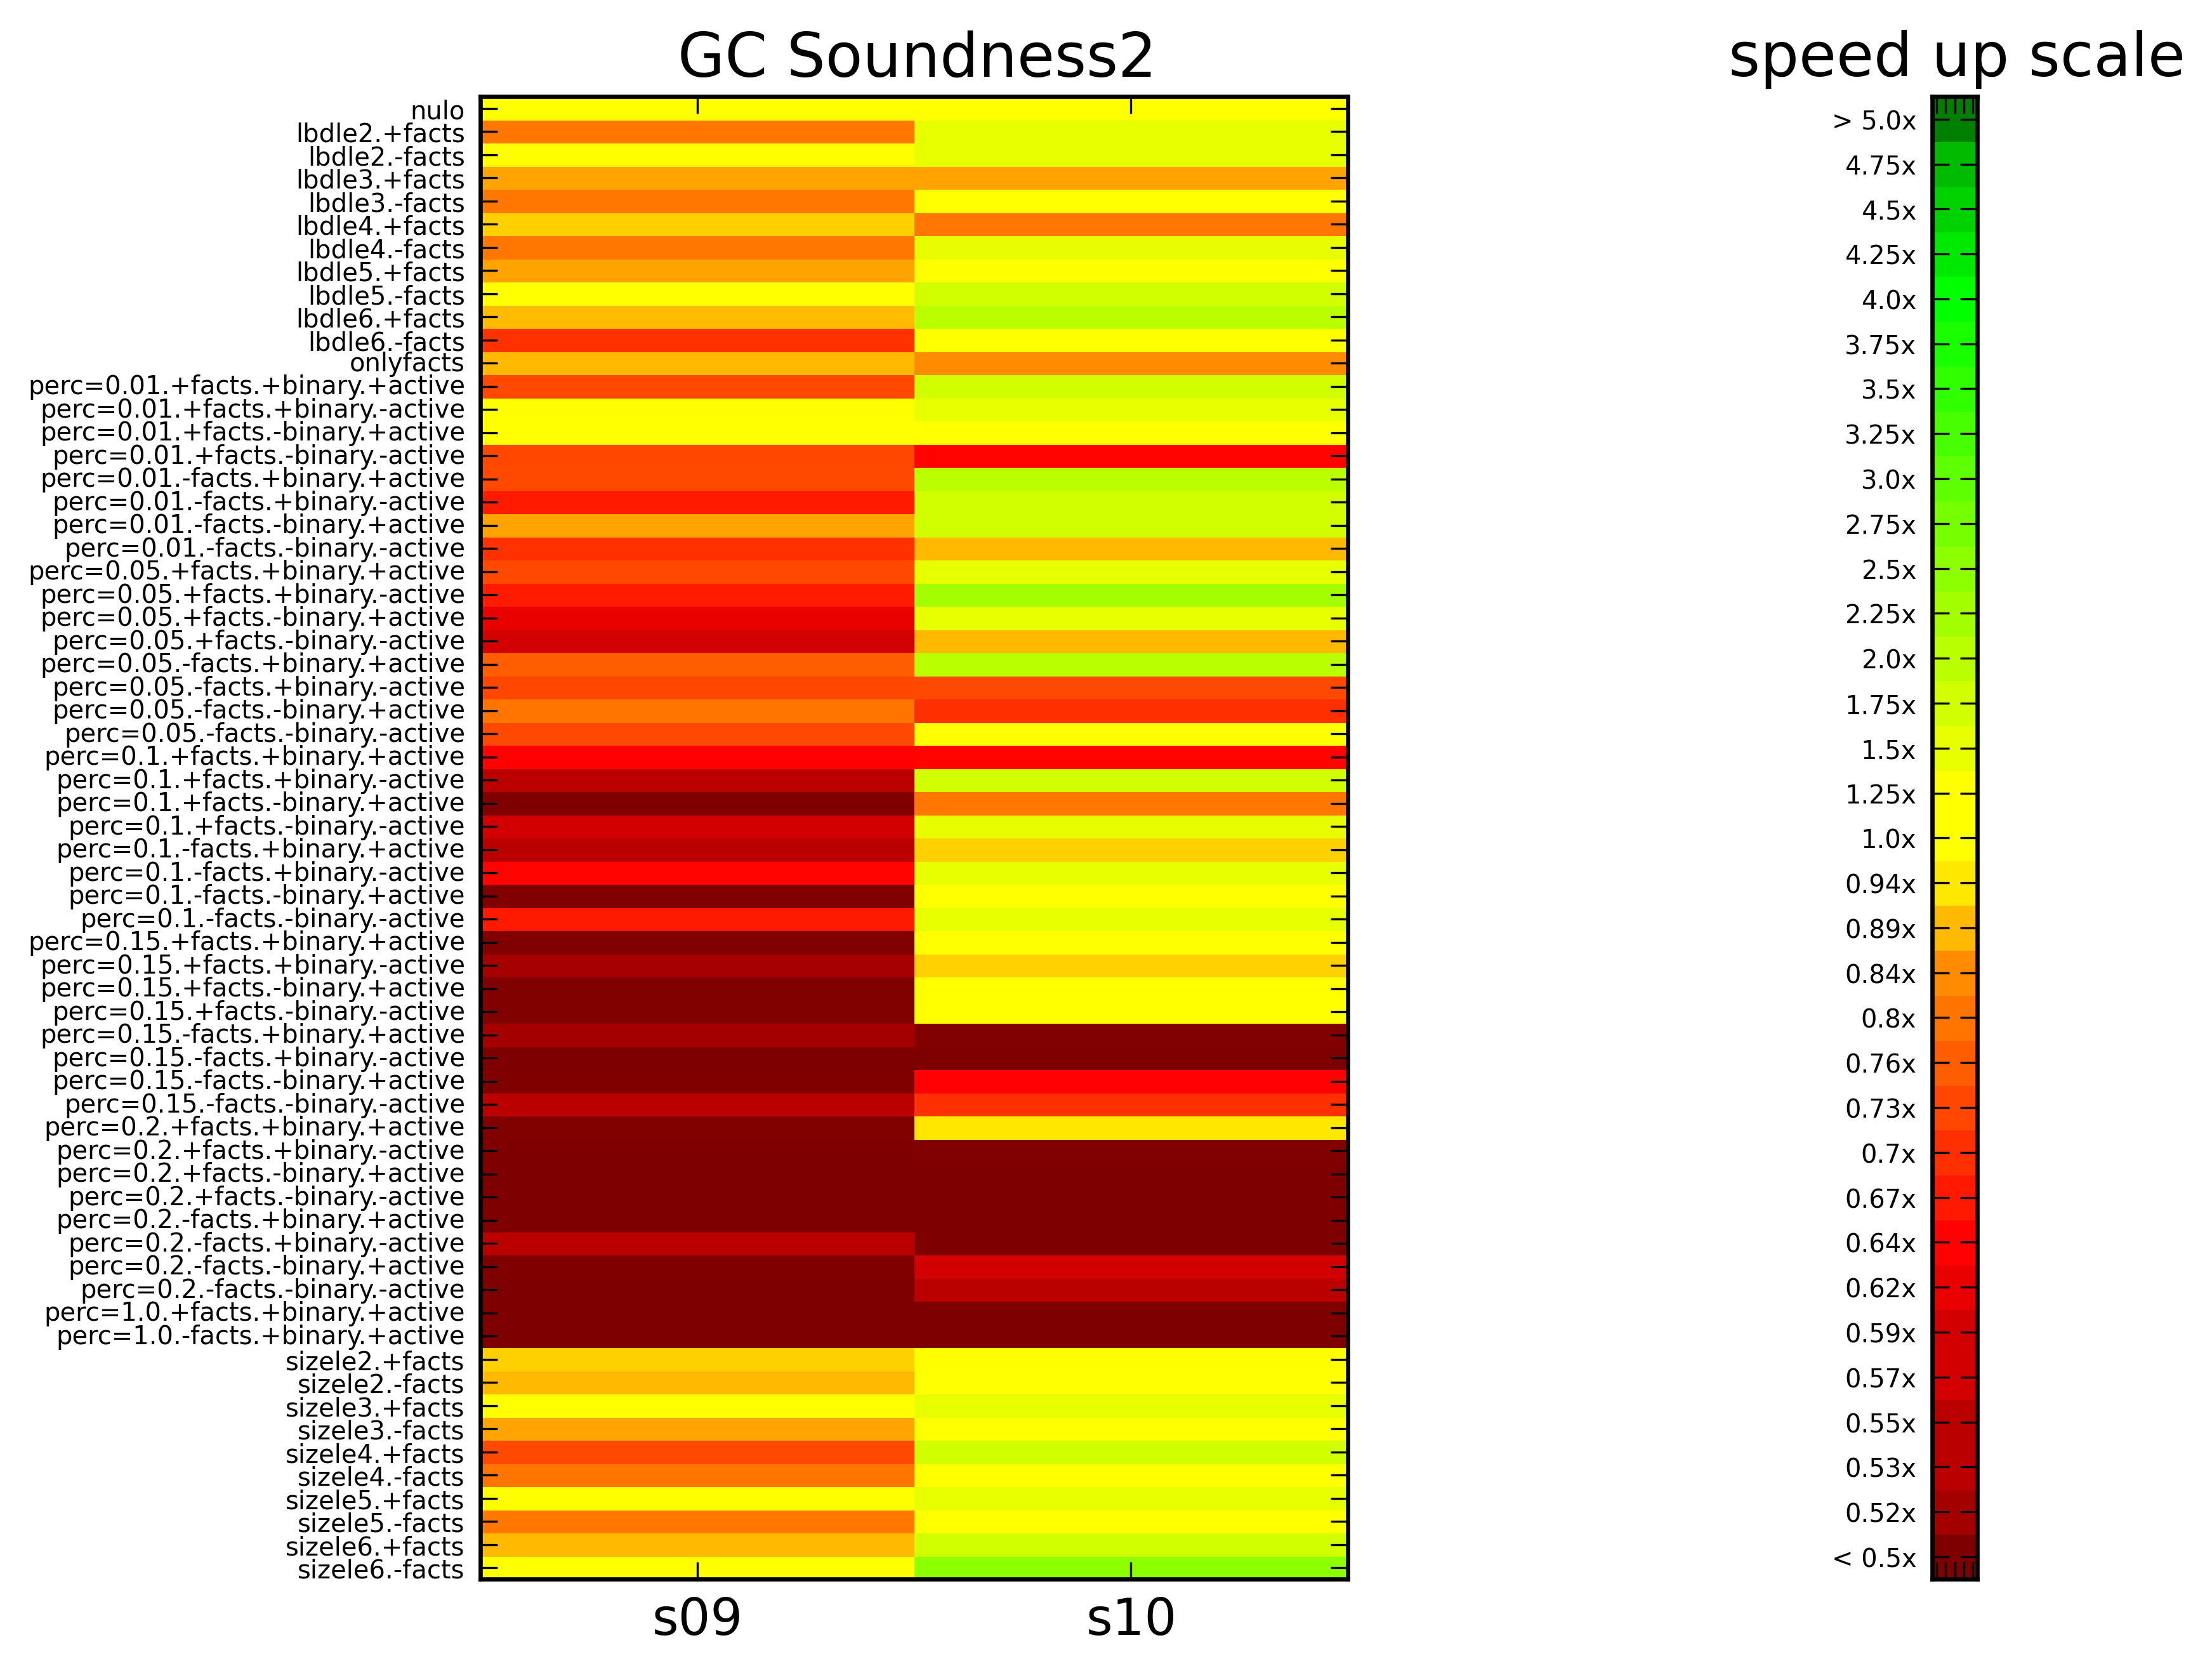
\includegraphics[width=\textwidth]{resultados/lossound_heat.png}
	\caption{Comparación de criterios de herencia para distintos \emph{scopes} para el problema GC Soundness2}
	\label{res:learnscopessoundness}
\end{figure}

\begin{figure}
	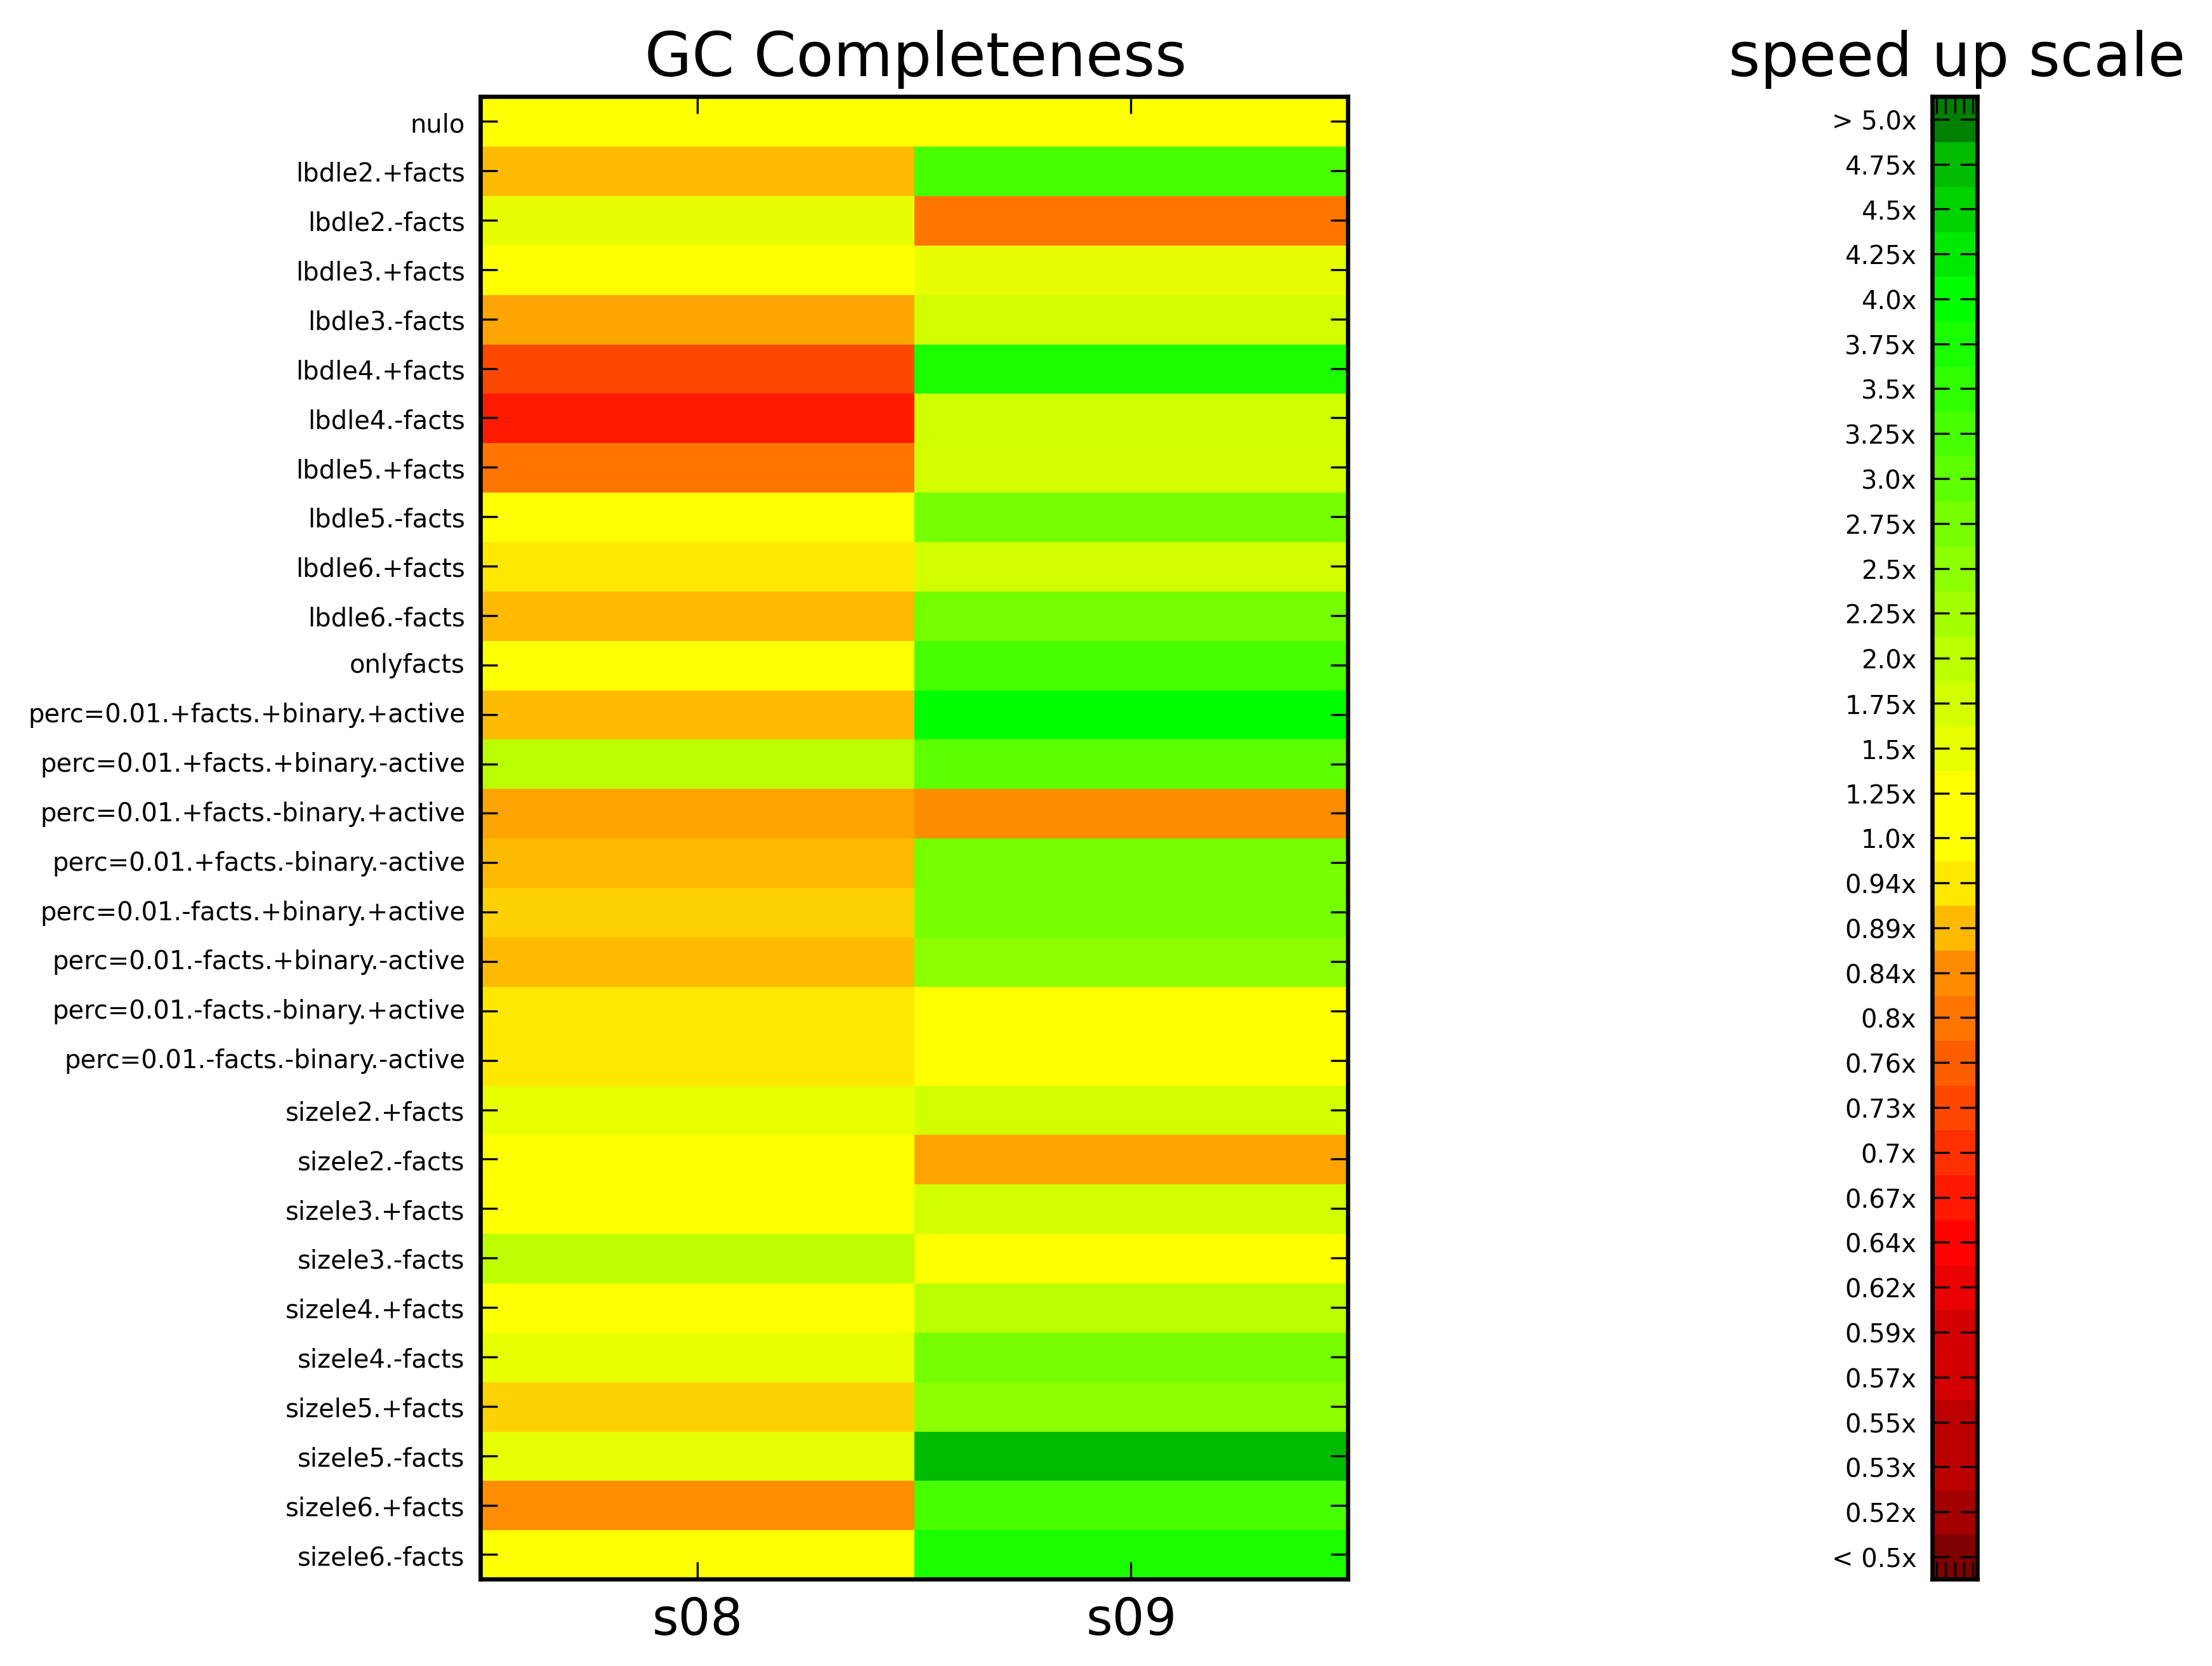
\includegraphics[width=\textwidth]{resultados/loscomp_heat.png}
	\caption{Comparación de criterios de herencia para distintos \emph{scopes} para el problema GC Completeness}
	\label{res:learnscopescompleteness}
\end{figure}

Nos interesa destacar dos observaciones de estos resultados. En primer lugar
parece existir una tendencia a que, a medida que aumenta el tamaño de un
problema, la herencia de cláusulas obtiene mejores resultados. Esto se observa
tanto en criterios que en \emph{scopes} chicos provocaron malos resultados,
como en criterios que provocaron buenos resultados.

También se observa cómo los resultados obtenidos por la herencia de cláusulas
varían considerablemente de problema en problema sin que exista una relación
evidente entre los problemas en los que esta metodología obtuvo buenos
resultados y problemas en los que no.

Por último se ve también que existe un subconjunto de los criterios probados
que resulta consistentemente negativo. Nos referimos a los criterios por
actividad que conservan el 10\% (o más) de las cláusulas aprendidas por el
padre.

\subsection{Discusión y conclusiones}


%!TEX root = tesis.tex
\chapter{Conclusiones y trabajo futuro}
\label{conclu}


\section{Conclusiones}

En el presente trabajo desarrollamos una herramienta de \ssolving paralelo y distribuido, orientada en particular a la verificación automática de propiedades sobre modelos formales de sistemas. Adoptamos un enfoque \emph{divide-and-conquer}, basado en una técnica conocida, para el particionamiento recursivo de subproblemas difíciles. Lo implementamos sobre una arquitectura original, dando respuesta a los aspectos cruciales de escalabilidad, usabilidad y automatización. Identificamos un factor limitante para la eficiencia del enfoque de particionamiento. Propusimos una solución basada en herencia de cláusulas aprendidas. Diseñamos e implementamos diversos criterios y evaluamos su desempeño.

\medskip

Las principales conclusiones respecto de la herramienta paralela y distribuida propiamente dicha son:

\begin{itemize}

\item La arquitectura resultó sólida y robusta, escalando sin inconvenientes al orden del centenar de \ws sobre decenas de equipos.

\item Para esa cantidad de \emph{hardware}, los (escasos pero cruciales) componentes centralizados no presentaron evidencia alguna de saturación. Incluso para corridas de problemas grandes se observó en esos puntos amplia capacidad ociosa.

\item Se identificaron correctamente los principales desafíos a resolver para lograr una operación 100\% automatizada. Se diseñaron soluciones pragmáticas, logrando convergencia y resultados satisfactorios para un banco de problemas con características disímiles, en distintos tamaños y grados de dificultad.

\end{itemize}



Las principales conclusiones respecto de la implementación y evaluación de cláusulas aprendidas en la herramienta distribuida son:

\begin{itemize}

\item La herencia de cláusulas aprendidas efectivamente permitió mejorar la eficiencia del análisis distribuido.

\item El grado en que eso ocurre parece depender fuertemente del problema.

\item Tanto para problemas donde la mejora es significativa como para aquellos donde no lo es, el grado de mejora tiende a aumentar junto con el tamaño de la instancia.

\item Es posible implementar un esquema de reuso de cláusulas aprendidas sin atentar contra la escalabilidad del sistema.

\item De los criterios de selección de cláusulas que evaluamos, el que logró mejores resultados globales fue aquel que retiene las cláusulas de tamaño menor o igual a 6, sin hechos.

\item Las mejoras en la eficiencia logradas gracias a la herencia de cláusulas aprendidas, si bien son significativas, no resuelven por completo el problema del retrabajo. Hay casos en que la eficiencia obtenida, a pesar de mejorar visiblemente respecto de la versión sin learning, sigue distando considerablemente del ideal lineal.

\end{itemize}



%[* Usando ese criterio, sobre los casos de estudio considerados el prototipo con herencia de cláusulas aprendidas logró un \emph{speedup} de ... [?]]




%Entre los aportes originales de esta tesis cabe destacar:
%
%\begin{itemize}
%
%\item \ldots
%
%\item \ldots
%
%\item \ldots
%
%\end{itemize}


\section{Trabajo futuro}

\subsubsection{Mejoras en la estrategia automatizada de toma de decisiones}

Uno de los aspectos más importantes a seguir refinando es la estrategia automática de toma de decisiones que hace posible la operación no supervisada del sistema. La versión actual logra evitar la mayor parte de los errores más evidentes, y así resulta capaz de llevar a buen puerto verificaciones breves, medianas y muy largas de propiedades muy diversas. Sin embargo, hay diversas capacidades que podrían ser mejoradas en futuras versiones.

Ante todo, los parámetros numéricos fijos restantes que se describieron en la sección~\ref{estrategia:implementada} deberían ser reemplazados por mecanismos autoajustables. También podrían refinarse los algoritmos y las métricas utilizadas para los mecanismos que ya son autoajustables. En particular:

\begin{itemize}
	\item Además de métricas directas (como la cantidad de problemas producidos y consumidos) y sus derivadas de primer orden (tasas de producción y consumo sobre tiempo), considerar también las de segundo orden (velocidad de estas últimas, i.e. aceleración de las primeras).
	\item Interpretar dichas métricas para determinar automáticamente la fase o etapa de la corrida en la que el sistema se encuentra (\emph{ramp-up}, meseta, \emph{ramp-down}, etc.), puesto que son varios los comportamientos que podrían beneficiarse variando en función de este conocimiento.
	\item Mejorar la estimación --y posiblemente la definición-- de ``progreso'', observando con mayor cuidado las métricas extendidas antedichas.
	\item El nivel de agresividad al partir --cuántas variables levantar, cuántos subproblemas generar como máximo en cada momento dado-- debería ser un parámetro dinámico que se autoajuste por retroalimentación en base al estado de las colas, la etapa actual de la corrida, etc.
	\item Utilizar información histórica para lograr algún grado de predecibilidad respecto de qué subproblemas tienen mayor probabilidad de ser los más difíciles de su camada, para así partirlos más temprano.
	\end{itemize}


\subsubsection{Evaluar la herramienta en \emph{clusters} más grandes}

Sería importante obtener acceso a (y cantidad suficiente de tiempo de cómputo en) grandes cantidades de \emph{hardware}. En primer lugar, para medir cómo escala el rendimiento conforme se agregan más y más \ws.

También sería interesante forzar la llegada al punto en que los componentes centralizados sí se conviertan en un factor limitante, para poder determinar si eso ocurre, por ejemplo, para cientos o para miles de \ws, y para observar si surgen otros factores limitantes que no hayamos imaginado.


\subsubsection{Diseñar y evaluar nuevos criterios de aprendizaje}

Ante todo sería necesario correr más experimentos, sobre una mayor diversidad de casos de estudio y para \emph{scopes} más grandes; esto último requiere abundante tiempo de cómputo.

Una ventaja en este sentido es el haber confirmado que ciertos criterios de aprendizaje no resultan beneficiosos. Dado que esos criterios solían ser los que más demoraban, su eliminación permitirá ahorrar tiempo de cómputo que podrá invertirse en la evaluación de nuevos criterios, diseñados en base a los que dieron mejores resultados.


\subsubsection{Análisis de conflictos, \emph{backjumping} y eliminación de subproblemas}

Sería importante pensar cómo llevar a cabo, a nivel distribuido, algo equivalente al análisis de conflictos que realizan las herramientas secuenciales (véase sección~\ref{backjumping}) de modo que permita lograr podas análogas a las que en secuencial se logran por medio del \emph{backtracking} no cronológico.

En la implementación distribuida, esto podría complementar el enfoque CDCL al permitirnos demostrar, durante o tras el análisis de un subproblema, que cierta cantidad de \emph{otros} subproblemas (como ser hermanos, primos o incluso ancestros) son necesariamente insatisfacibles, y así poder eliminarlos de las colas de pendientes y/o abortar sus análisis en curso, de haberlos.


\subsubsection{Interfaz más práctica para la toma de decisiones manual}

El mecanismo actual, basado en una consola interactiva, resulta de suma utilidad para intervenciones esporádicas en momentos clave de una corrida por lo demás automática. También permite controlar una corrida en forma totalmente manual, aunque esto no resulta del todo práctico debido a la gran cantidad de comandos involucrados y su extensión.

Sería mucho más amigable contar con algún tipo de interfaz gráfica en la que las tareas puedan arrastrarse entre \ws, partirse con un \emph{clic} sin necesidad de tipear largos identificadores de subproblema, etc.





\bibliography{tesis}{}
\bibliographystyle{plain}

\end{document}
